\documentclass{ieeeaccess}
\usepackage{cite}
\usepackage{amsmath,amssymb,amsfonts}
\usepackage{algorithmic}
\usepackage{graphicx}
\usepackage{caption}
\usepackage{url}
\usepackage{listings}
\usepackage{pdfpages}
\usepackage[english]{babel}
\usepackage{xcolor,colortbl}
\newtheorem{theorem}{Theorem}
\newtheorem{definition}{Definition}
\usepackage{scalerel}

\newcommand\neutral[1][.75]{\mathbin{\ThisStyle{\vcenter{\hbox{%
  \scalebox{#1}{$\SavedStyle\bullet$}}}}}%
}

\newcommand{\plus}{+}
\newcommand{\minus}{-}

\usepackage{textcomp}
\def\BibTeX{{\rm B\kern-.05em{\sc i\kern-.025em b}\kern-.08em
    T\kern-.1667em\lower.7ex\hbox{E}\kern-.125emX}}
\begin{document}
\history{Date of publication xxxx 00, 0000, date of current version xxxx 00, 0000.}
\doi{10.1109/ACCESS.2017.DOI}

\title{Privacy-preserving service provisioning using distributed networks}
\author{\uppercase{Stanis\l{}aw Bara{\'n}ski} \authorrefmark{1},
\uppercase{Julian Szyma{\'n}ski\authorrefmark{1} } 
 }

\address[1]{Department of Electronic, Telecommunication and Informatics, Gdansk University of Technology, Narutowicza 11/12 Gdansk Poland (e-mail: stanislaw.baranski@pg.edu.pl, julian.szymanski@eti.pg.edu.pl}

 

\tfootnote{The work has been supported partially by the founds of Department of Computer Architecture Faculty of Electronics, Telecommunications and Informatics, Gdańsk University of Technology.}

\markboth{S. Bara{\'n}ski, J. Szyma{\'n}ski : 
Anonymous provision of services via blockchain}
{S. Bara{\'n}ski, J. Szyma{\'n}ski : 
Anonymous provision of services via blockchain}

\corresp{Corresponding author: Stanislaw Baranski (e-mail: stanislaw.baranski@pg.edu.pl).}

\begin{abstract}
Service providers like lawyers, laboratories, auditors, or banks, to provide services, require customers to submit data often associated with their personal information, exposing their customers to privacy risks. However, most service providers use personal information merely for logistic operations like payments and communication and could provide services anonymously if other means of logistics exist.
We propose a anonymous fair exchange protocol for coordinating service provision using blockchain for both anonymous payments and proofs of existence and content-addressable network for results delivery.
% Less important
A service provider can employ our protocol to provide services without collecting personal information, enabling services currently based on unacceptable trust assumptions. 
% Even less important
Possible applications for this protocol include anonymous tests for drugs, venereal diseases, paternity, and steroids, or anonymous legal advice.
We provide the fairness analysis and well as the implementation of the protocol. We discuss further extensions to an anonymous delivery system, and a decentralized conflict resolution system.
\end{abstract}

\begin{keywords}
Anonymity, blockchain, fair-exchange, physical delivery, privacy, services
\end{keywords}

\titlepgskip=-15pt

\maketitle
\section{Introduction}
Service providers (SPs) like lawyers, laboratories, auditors, or banks, to provide services, require data that is often associated with the user identity.

Providing personal information exposes users to privacy risks, i.e. potential loss of control over personal information~\cite{smithInformationPrivacyResearch2011}.

Such personal information can be used deliberately or unintentionally
(e.g., by theft) for insider disclosure, unauthorized access, or commercial gains. For example, by reselling it to marketers, financial institutions, other businesses, government agencies, or even cybercriminals. Which in turn can lead to profiled advertisements or criminal activities like identity theft or illegal tracking and surveillance~\cite{smithInformationPrivacyResearch2011}.

Important individuals like influencers, politicians, or celebrities are especially vulnerable to this kind of attack as exposure of their health records, purchase habits, or legal documents can threaten their reputation, position or be used for blackmailing.

The privacy guarantee of the personal information is often based merely on trust assumptions and the security of the IT system. However, most SPs do not need personal information for any other reason than payment or communication, which should be considered secondary compared to actual service provision.

It would be desirable for the user to keep its identity private while still receiving the service. This could lead to reduced trust that users have to put on SPs and less responsibility borne by SPs.

Examples of services that would benefit from the anonymity property are:
\begin{itemize}
    \item Patients willing to take a test for drugs, venereal diseases, paternity or steroids have a strong incentive to keep the whole procedure private. Merely the fact that they took the test—without exposing the result—is suggestive enough to act as a premise in case of a conflict.

Especially celebrities, politicians, and public figures are prone to this kind of problem as such precedent can negatively influence their future career.

Currently, they have to risk that their personal details, materials, and results are stored securely and kept in private from any unauthorized actor (both curious employee and malicious attacker).

Our protocol allows taking such tests anonymously, eliminating the strong trust assumption put on the laboratories and their IT
systems.
\item People willing to take risky business activities may be willing to receive the risk estimation and prediction of possible personal repercussions of such action.

By exposing our identity we trust that the lawer will not use that information for harmful actions.

Our protocol would allow taking such advice anonymously, eliminating the strong trust assumption put on the lawyers and their IT systems.
\end{itemize}

% We observe
We observe that the issue of anonymous service provision can be seen as a problem of fair exchange where parties exchange some goods fairly, i.e., either both parties obtain the goods, or they both obtain nothing.

In our case, the customer who wants to use the service, exchanges his materials and money with the SP for the result of the service.

% Therefore we propose
We propose a protocol for anonymously provisioning services that require the delivery of physical materials. A service provider employing our protocol can provide services without collecting any personal information from customers.

In case of dispute, either due to exceeding deadlines or providing an incorrect result, the customer can disclose the whole interaction and prove to justice the misbehaviour of the SP.

To achieve these objectives, we use:
\begin{itemize}
    \item Blockchain (aka message board), to achieve fairness, i.e., as a means for proving that certain actions took place at a certain moment without the trusted third party (TTP).
    \item Anonymous payment methods, like cash or privacy-preserving cryptocurrencies, allowing customers to pay for the services anonymously.
    \item Content-addressable decentralised storage network (like IPFS) to anonymously provide results to customers. 
    \item Provable storage network (like Filecoin) to guarantee that the results are available to the customer even in case of the SP deny of service.
    \item Cryptography
    \begin{itemize}
        \item Symmetric encryption, to encrypt and decrypt results published on the public networks.
        \item Public-key cryptography, and Diffie-Helman key exchange (DHKE) to derive shared secrets for symmetric encryption.
        \item Digital signatures, to achieve authentication and non-repudiation of actions. 
    \end{itemize}
    
\end{itemize}


%\paragraph{Contributions}
We contribute to the field of fair exchanges by proposing a simple, practical, and anonymous protocol that does not rely on centralized TTP, but uses decentralized blockchain and
distributed content-addressable storage network.

Also, we support physical materials delivery, which was rarely targeted by other researchers or based on strong and unpractical assumptions.

Our protocol simultaneously provides five main properties:

\begin{itemize}
\item Anonymity: the customer stays anonymous to all external observers throughout the transaction.
\item Fairness: at each step of the protocol, both parties are incentivized to act accordingly to the protocol; otherwise, the misbehaving party ends up in a disadvantaged position.
\item Dispute resolution: at each step of the protocol, the customer can start a dispute and win the case if and only if the SP misbehaved.
\item Blockchain-obvious: the customer using our protocol does not need to interact with the blockchain directly; especially, he does not need to obtain funds and pay for the transaction fees, allowing the use of our protocol for non-technical users.
\item TTP-less: 
our protocol does not rely on a trusted third party to conduct transactions fairly. Only in case of a dispute, the centralised justice is involved, which can be instantiated either with courts and polices, or blockchain-based dispute resolution mechanisms as discussed in Section~\ref{sec:justice}.
\item Physical materials: our protocol allows providing not only digital but also physical materials to the service provider.
\end{itemize} 

Some authors have proposed blockchain-based fair-exchange systems that could be adapted to service provision; however, to our best knowledge, we are the first to propose a system that satisfies all five properties stated above. Especially anonymity and physical materials delivery were rarely addressed together, and if so, the protocol was based on TTP and impractical assumptions on banking system~\cite{birjoveanuAnonymityFairexchangeEcommerce2015} or did not address the conflict between parties~\cite{altawyLelantosBlockchainBasedAnonymous2017}.


%\paragraph{Organisation}
The remainder of this paper is organized as follows.
In section~\ref{sec:related-works} we review related works. 
Then, in section~\ref{sec:building-blocks} we discuss the concepts of dispute resolution system, self-sorveign identifiers, fairness, message board, anonimity, payment for services, storage network, result availability, anonymity and confidentiality.
Section~\ref{sec:protocol} describes how the protocol works in detail.
Section~\ref{sec:fairness-analysis} provides a fairness analysis of the proposed protocol.
Section~\ref{sec:discussion} discuss possible improvements. 
Finally, section~\ref{sec:conclusion} concludes the paper.


\section{Related Works}\label{sec:related-works}
In this section we review related works on fair exchange, anonymous, and physical delivery protocols. Then we outline the main differences between our protocol and the existing ones.

\subsection{Fair exchange, anonymity, and physical products delivery} 
\label{anonymity-and-fair-exchange-in-e-commerce-protocol-for-physical-products-delivery}

The most common application of anonymous fair exchange protocols is e-commerce. The problem is that the customer wants to buy a product from a merchant, but does not want to reveal his identity to the merchant. The problem gets even more challenging when physical products are involved.

Authors of~\cite{birjoveanuAnonymityFairexchangeEcommerce2015} proposed a protocol for fair exchange of physical products and electronic payments, which guarantee both customer and merchant anonymity. They achieve it by introducing online TTPs that validate coins and provide fair exchange guarantees.

The anonymity is ensured by assuming the existence of a source cabinet (SC), delivery cabinet (DC), and a trusted delivery agent who take a product from a SC and provide it to a DC.
Both cabinets provide access to the product by passwords to conceal
the identity of the customer and the merchant.

The protocol works as follows: \begingroup
\renewcommand{\labelenumii}{\arabic{enumii}.}

\begin{enumerate}
    \item Both parties agree on the purchase details.
    \item The customer buys a digital coin from his bank and validates it with the TTP.
    \item The customer sends the merchant the purchase order and the digital signature made by TTP on the encrypted coin.
    \item The merchant post the product to the SC.
    \item Delivery agent collects the product from the SC and posts it to the DC.
    \item Customer collects the product from the DC using a password.
    \item The customer checks if the product is the ordered one.
    \begin{itemize}
    \item[-] if yes 
        \begin{enumerate}
        \setcounter{enumii}{7}
        \item the customer sends the acknowledge to the DC and decryption key to the merchant.
        \item The merchant redeem the coins from the bank.
        \end{enumerate}
    \item[-] if no
        \begin{enumerate}
        \setcounter{enumii}{7}
        \item the DC is equipped with a video camera that records the moment when the customer opens the package and lets the customer signal the invalidity of the product, and so, sending the encrypted recording to the TTP. 
        \item the dispute is settled via TTP, optionally letting each party reveal its identity.
    \end{enumerate}
    \end{itemize}
\end{enumerate}
\endgroup

However, the protocol relies on strong assumptions, namely:

\begin{itemize}
    \item there exists trusted third party (TTP) and trusted delivery agent which do not misbehave or collude with any party;
    \item there exists an anonymous communication channel 
    \item the customer's and merchant's banks enable confidential transactions, and both share commit-buffer where the value is locked until the transaction is finished;
    \item all banks maintain a global list of coins' serial numbers to prevent double-spending problems;
    \item the SC and DC exist, and in both, the access is protected by a password;
    \item the DC is equipped with a video camera that records the moment when the customer opens the package and provides a way to submit the video to TTP in case of a dispute;
\end{itemize}


\subsection{Fair exchange and blockchain}

The issue of TTPs in fair exchange protocols has been solved by the usage of decentralised networks, especially blockchain technology.

The simplest example of blockchain-based fair exchange protocol is certified electronic mail protocol in which neither the sender can deny sending the mail, nor the receiver can deny receiving it. As the service is widely used in the paper world, achieving it for e-mails has not yet met the agreement across the scientific community. The main problem was the dependency of TTP, which significantly reduced the performance, security, and robustness of such protocols. The protocols that do not use TTP struggle with high computation and communication overhead~\cite{hinarejosSolutionSecureCertified2019}.

Authors of ~\cite{hinarejosSolutionSecureCertified2019} replaced the TTP with blockchain (concretely Bitcoin blockchain as a reference implementation) that acts as a secure, verifiable, and decentralized TTP.

The idea behind certified e-mails and any other fair exchange protocols is following:
\begin{enumerate}
    \item The sender sends encrypted and signed message to the receiver.
    \item The receiver returns a proof of delivery (a signature) of the encrypted message to the sender.
    \item The sender publishes proof of delivery and the decryption key on a blockchain (or TTP in general).
    \item The receiver decrypts the encrypted message using the published decryption key.
\end{enumerate}

The non-repudiation requirement is achieved by the receiver sending the proof of delivery prior to having access to the decrypted message and the sender publishing the decryption key together with the proof of delivery on the blockchain (or TTP) so that the receiver can deny neither receiving the message nor having access to the decryption key—because it is publicly available.

In this case, the role of blockchain is to certify the existence of the decryption key at a certain time.

\subsection{Fair-exchange, blockchain, and decentralized dispute resolution}
\label{themis-towards-decentralized-escrow-of-cryptocurrencies-without-trusted-third-parties}

Themis~\cite{mengThemisDecentralizedEscrow2019} is a fair exchange protocol that uses blockchain instead of TTP. It provides an escrow service for the secure exchange of cryptocurrencies and digital goods. Also, it provides a decentralized dispute resolution system for resolving conflicts.

Two parties say, Alice and Bob, can create an escrow by generating
2-of-2 (not 2-of-3 as it is other TTP-based systems) threshold account
using Thresh-Key-Gen protocol. Alice and Bob generate secret keys
\(x_A\) and \(x_B\) accordingly, the shared account public key becomes
\(y = g^{x_A+x_B}\); only the access to both Alice's and Bob's secrets
grants access to the shared account.

Then, both Alice and Bob take their keys and split them into
\(n=2t+1\) secret shares using Shamir Secret Shamir protocol, where
\(n\) is the number of mediators that participate in the decentralized
network and \(t+1\) becomes the threshold of a sufficient number of mediators to reconstruct the secret key.

Next, both Alice and Bob, take their key shares, and encrypt each
\textit{i}-th key share using public key of \textit{i}-th mediator. As a result
Alice's secret \(x_A\) becomes \({c^A_1, c^A_2,...,c^A_n}\), and Bob's
secret \(x_B\) becomes \({c^B_1, c^B_2,...,c^B_n}\), where
\(c_i = E_{M_i}(P_i)\) is the encrypted \(i\)-th key share using
\(i\)-th mediator public key \(M_i\).

Next, both Alice and Bob exchange the sets of encrypted key shares with
each other, and send funds to the escrow account.

The escrow is secure as long as \(t+1\) of mediators does not collude,
which would let them recreate both \(x_A\) and \(x_B\). To ensure
that parties exchange actual key shares, they send witnesses
generated with the Feldman VSS scheme and zero-knowledge proofs to guarantee the consistency between witnesses and key shares.

In case of dispute, the decentralized network of mediators settle the conflict and grand one winning party, the other party secret key,
letting him withdraw the funds.

The monetary incentivization and reputation system guarantee the honesty of mediators.

\subsection{Blockchain, anonymity, and physical delivery}\label{lelantos-a-blockchain-based-anonymous-physical-delivery-system}

Lelantos~\cite{altawyLelantosBlockchainBasedAnonymous2017} is a blockchain-based anonymous
physical delivery system. The protocol achieves anonymity by employing onion routing (similar to the Tor network) to connect physical delivery providers. The whole route from a merchant to a customer is split into multiple steps, and each step is undertaken by the different randomly selected delivery providers. As long as the delivery providers do not collude, a merchant neither can learn the identity nor destination address of the customer.

Onchain smart-contract is used to coordinate the whole process and
mediate communication between customers and delivery providers.

However, since the system uses Ethereum, it achieves pseudonymity rather than anonymity (see section~\ref{sec:pseudo-anon}). Also, the protocol does not cover disputes between the parties.

\subsection{Comparision}

We considered only protocols that achieve fair exchange as it is the fundamental feature of such protocols.

Bîrjoveanu, 2015~\cite{birjoveanuAnonymityFairexchangeEcommerce2015} is the closest to our protocol, however it uses TTP and does not consider dispute between parties.

Hinarejos et al., 2019~\cite{hinarejosSolutionSecureCertified2019} is the simplest protocol that replaces TTP with blockchain. However, it does not consider anonymity, dispute between parties nor physical material exchange.

Meng et al., 2019~\cite{mengThemisDecentralizedEscrow2019} improves the previous protocol by the crownsource dispute resolution system. However it does not take anonimity into consideration.

Altawy et al., 2017~\cite{altawyLelantosBlockchainBasedAnonymous2017} is a blockchain-based protocol that does not provide dispute resolution, but provides anonymous physical delivery by using onion routing and anonymous blockchain interaction assuming unlinkability between pseudonyms and real identities.


Our protocol achieves stronger anonymity guarantees. Namely, we achieve anonimity by using either cash or privacy-preserving blockchains. Moreover, our protocol does not require a customer to submit any transaction to the message board, which may be the weakest link in the anonymity of aforementioned protocols.

Our protocol does not use its own delivery system. We assume that there is a way to anonymously deliver a package either via SP's drop box, or trusted party.

Also, our protocol does not provide its own dispute resolution mechanism as Themis does. However, we assume the existence of an abstract justice which accepts evidences and ., which can be instantiated with either local court or police, or one of the available online dispute resolution services like Themis~\cite{mengThemisDecentralizedEscrow2019}, Kleros~\cite{bergollaKlerosSociolegalCase2022}, Aragon Court\footnote{https://aragon.org/aragon-court}, or others~\cite{allenGovernanceBlockchainDispute2019}.

The comparision of the protocols is presented in table~\ref{tab:comparision}.


\begin{table}
  \newcommand{\YES}{\cellcolor{green!50}Yes}
  \newcommand{\ID}{\cellcolor{green!25}Identity}
  \newcommand{\PSEUDO}{\cellcolor{green!25}Pseudonym}
  \newcommand{\ANON}{\cellcolor{green!50}Anonymity}
  \newcommand{\NO}{\cellcolor{red!50}No}
  \newcommand{\TTP}{\cellcolor{red!50}TTP}
  \newcommand{\BC}{\cellcolor{green!50}Blockchain}
  \caption{Related work comparision}
  \label{tab:comparision}
  \setlength{\tabcolsep}{3pt}
  \begin{tabular}{|p{38pt}|p{32pt}|p{38pt}|p{35pt}|p{37pt}|p{30pt}|}
  \hline
  Protocol & Fair exchange & Anonymity & Dispute resolution & Trust & Physical delivery \\
  \hline
  Bîrjoveanu, 2015~\cite{birjoveanuAnonymityFairexchangeEcommerce2015} & \YES & \YES & \NO & \TTP & \YES \\
  \hline
  Hinarejos et al., 2019~\cite{hinarejosSolutionSecureCertified2019} & \YES & \NO & \NO & \BC & \NO \\
  \hline
  Themis~\cite{mengThemisDecentralizedEscrow2019} & \YES & \NO & \YES & \BC & \NO \\
  \hline
  Lelantos~\cite{altawyLelantosBlockchainBasedAnonymous2017} & \YES & \PSEUDO & \NO & \BC & \YES \\
  \hline
  This paper & \YES & \YES & \YES & \BC & \YES \\
  \hline

  \end{tabular}
\end{table}
 
\section{Building Blocks}\label{sec:building-blocks}
\subsection{Dispute resolution system}

Disputes are an inevitable part of all human transactions. Whether intentional or accidental, the system should prevent violation of agreed contract rules or local jurisdiction. The rules are specified by law and implemented by the police.

The vision of smart contracts was to replace the legal contract with
programmable and autonomous contracts. The smart contract code encompasses the contract's specifications, hence the slogan \textit{code as a law}. Moreover, smart contracts are automatically executed merging together the gap of law and its enforcment by police~\cite{allenGovernanceBlockchainDispute2019}. However, the blockchain paradigm has its limitations. 
 
Blockchain can assure the correctness of data existing only on the blockchain. The problem arises in the contact between blockchain and the real world, when we want the smart contract to decide based on some input from outside the blockchain. The technique of providing real-world data to the blockchain is called oracle. Oracle provides data based on a decentralized network of mediators; therefore, the trust is also decentralized~\cite{breidenbachChainlinkNextSteps2021}.

Some oracles provide the data like weather, soccer match result, stock
price, train delay, election results, others—and they are the ones we
are interested in—provide the settlement of a submitted dispute.

Themis~\cite{mengThemisDecentralizedEscrow2019} besides providing fair exchange protocol,
also offers a semi-autonomous decentralized dispute resolution system that complies with the Web3 postulates of a decentralized web. Themis
resolve disputes by a set of voluntary anonymous mediators participating
in voting and deciding whether a party misbehaved. The honesty of
mediators is achieved by the monetary incentivization and reputation
system.

Kleros~\cite{bergollaKlerosSociolegalCase2022} is a smart contract deployed on the Ethereum platform that mimics in a decentralized and autonomous way how the court works in real life. In Kleros, every process of a dispute like gathering evidence, selecting jurors, rewarding the winning party is automated by a set of smart contracts. Like Themis, the honesty of the agents voting in a case is achieved by game-theoretical economic incentives.

Such a decentralized, voluntary, and anonymous dispute resolution system might work for simple contracts violations like an eBay seller sending broken or wrong products or an Airbnb apartment being inadequate to the photos in the offer. However, it is hard to realize such decentralized evaluation of heath or legal services quality when expertise and privacy concerns are taken into account. Therefore, in our protocol, we take the more conservative approach and resolve disputes using local
justice system (police or court).

Possible directions toward semi-autonomous decentralized resolution system are discussed in Section~\ref{sec:decentralised-justice}.

\subsection{Fairness}\label{fairness}

In case of dispute, the customer can prove to justice (police or court) convincing evidence for the honesty of the customer and misbehaviour of the SP. 
Because the customer is anonymous, the SP can not start a dispute---there is no means to identify the customer.

To mitigate the issue, we designed the protocol so that the SP who follows the protocol is always in an advantaged position; therefore, she has no reason to start a dispute. On the other hand, the customer can start a dispute at any time of the protocol, but only the actual misbehaviour of the SP makes him win the case.

Abstracting from the services the SP is providing, each party should be able to prove its honest behaviour in case of a dispute. We introduce three proofs that should be disclosed to justice in case of a dispute:

\begin{enumerate}
    \item Proof of delivery ($\mathrm{PoD}$) is a confirmation issued by the SP to the customer that proves that the customer has delivered to the SP a complete (according to the SP requirements) package, and the SP accepted it. It consists of the current time, the deadline to pay for the transaction, the deadline to provide a result of the service, randomly generated number uniquely identifying the transaction, and the SP's signature guaranteeing non-repudiation. The formal definition of the $\mathrm{PoD}$ is presented in section ~\ref{proof-of-delivery}.
    
    \item Payment $\mathrm{attestation}$ is confirmation that the customer has paid for the transaction at a certain time. The actual implementation depends on the particular cryptocurrency and is discussed further section~\ref{payment-for-services}.
    
    \item Proof of provision ($\mathrm{PoP}$) is proof that the SP published the result at a certain time. It defends the SP in case the customer unjustly starts a dispute after the result has been published. It consists of a content identifier as specified in section ~\ref{storage-network}, the $\mathrm{nonce}$ uniquely identifying the transaction previously generated in $\mathrm{PoD}$, and the SP's signature guaranteeing authentication. The connection between $\mathrm{PoP}$ and the result is created by the content identifier ($\mathrm{cid}$) that uniquely identify the result (it is some kind of a hash of the result) such that the result can not be forged after the $\mathrm{PoP}$ has been published.
\end{enumerate}

\subsection{Message Board}\label{sec:message-board}
The proof of provision that we coined for the purpose of this protocol is generally called the proof of existence~\cite{ProofExistenceOnline, crespoStamperyBlockchainTimestamping2017, ChainpointBlockchainProof}.

The idea behind proof of existence is to certify that some information
has existed at a certain moment, in such a way that nobody can
undermine its existence, integrity, and ownership (also called the
non-repudiation requirement).


We need this functionality for two reasons: (1) communicate the existence of the result to the customer to whom the SP have no other communication medium as the customer stays anonymous; (2) let the SP to proof the publication of the result within the agreed with customer deadline. 

By publishing the $\mathrm{PoP}$ on the blockchain, the SP can not falsify the time at which the result has been provided because the block creation time proves that. Blockchain acts as a global clock that securely timestamps everything that gets into the block, so the $\mathrm{PoP}$ that was included in a block will be associated with the time when the block has been created. Moreover, since the blockchain is public, everyone (including justice) can be convinced that the SP indeed published the result at that time.

Without such proof, there would be no other means to settle the conflict between the customer claiming the result has not been published and the SP claiming the result has been published within the deadline.

Depending on the context the platform of achieving it is called bulletin board~\cite{achenbachImprovedCoercionresistantElectronic2015}, trusted timestamping~\cite{gippDecentralizedTrustedTimestamping2015}, or message board~\cite{hinarejosSolutionSecureCertified2019}. In this work, we call it a message board.

We keep the protocol general enough to be implemented using any existing technology to provide message board service, assuming it is decentralized and supports subscribing for the upcoming proofs from a particular address.

\subsection{Anonymity, pseudonomity, and confidentality}\label{sec:pseudo-anon}

Privacy is a concept used in almost all social sciences like philosophy, psychology, sociology, and legal. The multidisciplinary nature leads to ambiguous definitions~\cite{smithInformationPrivacyResearch2011}. For our work, we rely on more concrete definitions, i.e.~confidentality and anonymity.

Confidentiality is the ability to hide the details of an action from others. Alternatively, we can say that the system guarantees confidentiality if, for all observers, everything they can say about the action is the fact that it happened and nothing more.

Anonymity is the ability to hide one identity from others. More precisely, the inability to correlate actions performed within the system with the user's identity. Alternatively, we can say that the system guarantees anonymity if, for all observers, the actions are equally likely to be associated with any user of the system. However, anonymity is a spectrum rather than a dichotomous classification. One method of quantifying the level of anonymity is \textit{k}-anonymity proposed in~\cite{sweeneyKanonymityModelProtecting2002}. It measures the user's anonymity by the number of other users from whom the user can not be distinguished. Concretely, the user is \textit{k}-anonymous if his actions are equally likely associated with \textit{k}-1 other users; the larger \textit{k}, the higher anonymity.

Some anonymity techniques can be deployed on non-anonymous blockchains. The so-called mixers gather users into an \textit{anonymity set}, which then collude together to launder transactions in such a way that to an observer, the likelihood of the sender of each transaction is equiprobable for any user from the anonymity set.

Some systems guarantee pseudonymity rather than anonymity. Pseudonymity allows users to hide their real identity behind the pseudonyms. Despite the whole system being transparent and allowing linking actions to pseudonyms, the system is considered anonymous as long as the link between pseudonyms and real identities is secret. This assumption is hard to satisfy in practice, as the KYC (Know Your Customer) and AML (Anti Money Laundering) regulations require users to reveal their real identity to cryptocurrencies exchanges, making the user's anonymity dependent on the security of the IT system. Moreover, some correlations can be inferred merely by the analysis of transactions \cite{androulakiEvaluatingUserPrivacy2013, oberStructureAnonymityBitcoin2013}.

The figure ~\ref{fig:anonymity-diagram} ilustrate relations between these terms.

\begin{figure}[h!]
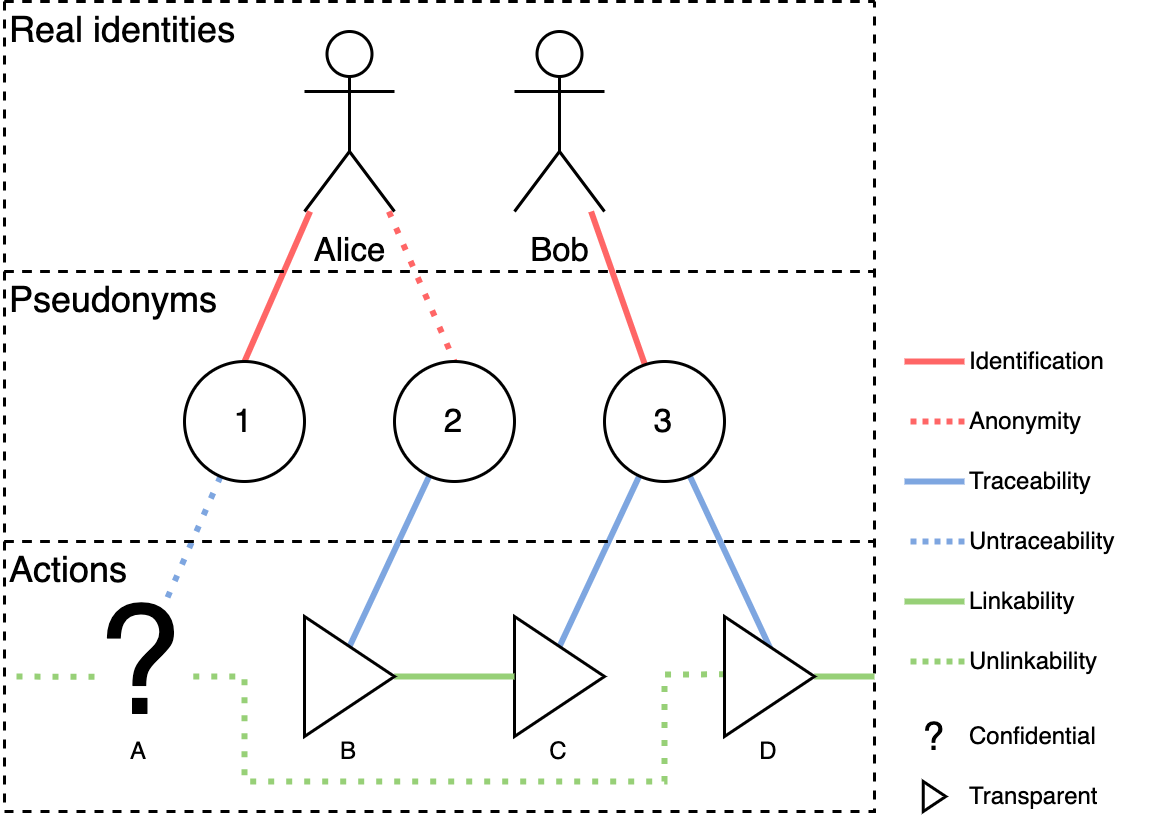
\includegraphics[width=9cm]{anonymity-diagram.png}
\centering
\caption{Let us assume Alice to be the customer willing to keep her identity anonymous and Bob to be the public SP. Alice controls two addresses, 1 and 2; the connection between her real identity and the first address has been compromised, and therefore the identification is possible; the connection between the second pseudonym is still unknown therefore anonymous. Alice takes two actions; the first one from the compromised address and the second one from the anonymous one. The first action is confidential; therefore, even though the pseudonym has been compromised, the action can not be associated with Alice. The second action is transparent; therefore, Alice maintain her anonymity as long as the connection to the second pseudonym is concealed.}

\label{fig:anonymity-diagram}
\end{figure}

The privacy-preserving blockchains are the ones that maintain anonymity via untraceability and (ideally) unlikability, not via the assumption that the connection between an address (pseudonym) and the real identity is concealed.   

Examples of blockchains that natively support confidential transactions are: Monero~\cite{vansaberhagenCryptoNote2013} (via Ring Signatures~\cite{noetherRingSignatureConfidential2015} and Bulletproofs~\cite{moneroBulletproofsMoneropediaMonero, bunzBulletproofsShortProofs2018}), ZCash~\cite{ben-sassonZerocashDecentralizedAnonymous2014} (via zkSNARK~\cite{ben-sassonSNARKsVerifyingProgram2013}), and Grin~\cite{fuchsbauerAggregateCashSystems2019} (via Mimblewimble~\cite{jedusorMIMBLEWIMBLE2016}).

Overly techniques that achieve anonymity on top of non-privacy-preserving blockchains are: Ethereum's Tornado Cash\cite{pertsevTornadoCashPrivacy2019} (via zkSNARK~\cite{grothSizePairingbasedNoninteractive2016} and MiMC~\cite{albrechtMiMCEfficientEncryption2016}), Bitcoin's Wasabi\footnote{https://wasabiwallet.io/} (via CoinJoin \cite{maxwellCoinJoinBitcoinPrivacy2013}).

\subsection{Payment for services}\label{payment-for-services}
Transactions between customers and SPs must be pegged to prevent proving one payment for multiple transactions. In other
words, we need a mechanism that uniquely associates a payment with the corresponding transaction.

Depending on a cryptocurrency, the link can be created in different
ways:
% continue reading from here
\begin{itemize}

\item separate address: each transaction derives a new address uniquely associated with the transaction. Such addresses can be derived using Hierarchical Deterministic Wallets (BIP-32)\footnote{https://github.com/bitcoin/bips/blob/master/bip-0032.mediawiki}.
\item memo: the payments are sent to one SP account but contain an extra field named ``memo'' filled with the unique number provided by the SP in $\mathrm{PoD}$. Each payment containing such value in the memo is considered to pay for the transaction. In case of a dispute, revealing both the payment memo and the $\mathrm{PoD}$ proves the connection.
\end{itemize}

Both approaches have some advantages and disadvantages, but our protocol can abstract them away by treating them as some randomly generated unique number, often called \textit{nonce} (number once). The actual implementation depends on a particular blockchain.

In case of a dispute, there must be a way to prove to the justice that the customer has paid for the transaction. As the proof of transaction is trivial in transparent and trackable blockchains, it gets more complicated when it comes to anonymous blockchains. Monero allows proving and checking payments via dedicated API \cite{MoneroHowProve}. ZCash provides a mechanism called Payment Disclosure \cite{daviesIntroductionPaymentDisclosure2017}.

\subsection{Storage network}\label{storage-network}
Once the SP finishes its service, she has to provide the result to the customer. The most natural approach would be to send the result via e-mail or some dedicated platform. However, since the customer wants to stay anonymous and so does not want to expose his e-mail address nor IP address. Moreover, the SP should prove that the result has been provided before the deadline, which brings us to the issue of proof of existence discussed in section ~\ref{sec:message-board}.

One approach would be to post the result into a blockchain. However, storing data on a blockchain is very expensive. The most common workaround (\cite{shahidBlockchainBasedAgriFoodSupply2020, wangAuditableProtocolsFair2019, chenImprovedP2PFile2017}) is to publish the data on a content addressable peer-to-peer storage network like IPFS~\cite{benetIPFSContentAddressed2014}. Then, publish on the blockchain just the content identifier ($\mathrm{cid}$) that uniquely points to the content stored on IPFS.

We take the same approach. Once the SP creates the result, she encrypts it using the previously provided encryption key and uploads it to the IPFS network.
%TODO: write about DHKE encyption

To increase anonymity, the customer should use standard techniques to hide its IP address, such as gateway, VPN, proxy, or onion routing.

\subsection{Separation of concerns}
We could use one blockchain to achieve all of these three roles: (i) anonymous payments, (ii) message board, (iii) storage network.

While most blockchains could provide the message board functionality, anonymous payments are not as prevalent. Especially a provable storage network is a functionality of a few specialized blockchains.

Instead of searching for one blockchain that provides all the functionalities, we allow the protocol to use separate blockchains for each role. If a suitable blockchain arises, it can play more than one role.

At the time of writing, we see the following technologies that fulfil the requirements of each role:

\begin{enumerate}
\def\labelenumi{\arabic{enumi}.}

\item Anonymous payments: Monero \cite{vansaberhagenCryptoNote2013}, ZCash
  \cite{ben-sassonZerocashDecentralizedAnonymous2014}, Grin \cite{fuchsbauerAggregateCashSystems2019},
  Tornado Cash \cite{pertsevTornadoCashPrivacy2019}.
\item Message board: Stampery \cite{crespoStamperyBlockchainTimestamping2017}, Proof of Existence
  \cite{ProofExistenceOnline} (Bitcoin blockchain), Chainpoint
  \cite{ChainpointBlockchainProof} (Bitcoin blockchain), or any other blockchain that
  supports attaching extra data along the transaction.
\item Storage network: IPFS \cite{benetIPFSContentAddressed2014}, Filecoin
  \cite{protocollabsFilecoinDecentralizedStorage2017}, or Ethereum's
  Swarm\cite{teamSWARMStorageCommunication2021}.
\end{enumerate}

\section{The Protocol}\label{sec:protocol}
In this section we propose an abstract protocol for anonymous service provisioning without any assumptions about the underlying technologies. We define the requirements for each role and leave the choice of the technology to the developer. Later in the paper (section~\ref{sec:experiments}) we describe our implementation used for conducting experiments.

\subsection{Prerequisites}

\begin{itemize}
\item There exists PKI infrastructure:
    \begin{itemize}
        \item The customer and the SP have their key pairs consisting of secret key $\mathrm{sk}(\mathrm{party})$ and public key $\mathrm{pk}(\mathrm{party})$, where $\mathrm{party} \in \{\mathrm{C}, \mathrm{SP}\}$ for the customer and the SP.
        \item Both the customer and the SP can create and verify digital signatures created by the customer $\mathrm{sig}_{\mathrm{sk}(\mathrm{C})}$ and the SP $\mathrm{sig}_{\mathrm{sk}(\mathrm{SP})}$.
        \item The SP's public key $\mathrm{pk}(\mathrm{SP})$ is publicly known.
    \end{itemize}
    
\item Both the customer and the SP:
    \begin{itemize}
        \item use common symmetric encryption $\mathrm{E}_\mathrm{key}(\cdot)$ and decryption $\mathrm{D}_\mathrm{key}(\cdot)$ operations.
        \item have access to anonymous payments blockchain, message board, and storage network.
    \end{itemize}

\item The SP:
    \begin{itemize}
        \item accepts packages from unknown customers.
        \item accepts payments with anonymous cryptocurrencies as described in section~\ref{payment-for-services}.
    \end{itemize}
    
\item Justice:
    \begin{itemize}
        \item accepts as evidence in a dispute the $\mathrm{PoD}$, $\mathrm{PoP}$, and payment $\mathrm{attestation}$ as described in section~\ref{fairness}.
    \end{itemize}

\item Anonymous payments blockchain:
    \begin{itemize}
        \item supports anonymous, i.e., untraceable and (ideally) unlinkable transactions as specified in section~\ref{sec:pseudo-anon}.
        \item supports uniquely identifying transaction either via separate address, memo field, or other similar mechanisms as described in section ~\ref{payment-for-services}. 
    \end{itemize}

\item Message Board:
    \begin{itemize}
        \item supports transactions of sizes up to $\mathrm{PoD}$ and $\mathrm{PoP}$.
    \end{itemize}

\item Storage network:
    \begin{itemize}
        \item allows for content retrieval via content identifier $\mathrm{cid}$ (usually a hash of the content).
        \item allows for anonymous content retrieval.
        \item guarantee that the content will be available for the duration of the agreement.
    \end{itemize}
\end{itemize}

\subsection{Messages}\label{messages}
In this section, we describe the messages exchanged between the parties of the protocol.

\vspace{5mm}

\noindent \textbf
{Package}\label{package} is a physical container prepared by the customer encompassing all $\mathrm{materials}$ required by the SP to provide the service, randomly generated provision identifier used to anonymously track the provision throughout the protocol's steps, and the customer's public key $\mathrm{pk(C)}$ used to encrypt the result published on the public storage network.

$$\mathrm{pkg} \equiv (\mathrm{materials}, \mathrm{provisionID}, \mathrm{pk(C)})$$

where:

\begin{itemize}

\item $\mathrm{materials}$ - are the materials required to provide the service, for example, samples of urine, blood, stool, saliva; legal documents, CDs, emails, photos, bank statements; or any other kind of materials depending on the service.
\item $\mathrm{provisionID}$ - a randomly generated provision identifier, used to anonymously track the provision throughout the protocol's steps.
\item $\mathrm{pk(C)}$ - customer's public key used to encrypt the result published on the public storage network.
\end{itemize}

\noindent \textbf
{Proof of delivery ($\mathrm{PoD}$)}\label{proof-of-delivery} is an attestation to the fact that the customer has delivered a correct (according to the SP requirements) package to the SP, and the SP has accepted it.

It is also an agreement between the customer and the SP, as it includes agreed upfront deadlines of actions, and a payment method.

$\mathrm{PoD}$ is published on the message board by the SP.

\begin{eqnarray}
\mathrm{PoD} & \equiv & (\begin{array}[t]{l}\mathrm{T}_\mathrm{issue}, \mathrm{T}_\mathrm{pay}, \mathrm{T}_\mathrm{provide},\\ \mathrm{address}, \mathrm{provisionID}, \mathrm{pk(C)}, \mathrm{sig}_\mathrm{SP} \; )\end{array}
\end{eqnarray}

% \begin{eqnarray}
%   \quad L_{\mathrm{H}}(H) & \equiv & (\begin{array}[t]{l}H_{\mathrm{p}}, H_{\mathrm{o}}, H_{\mathrm{c}}, H_{\mathrm{r}}, H_{\mathrm{t}}, H_{\mathrm{e}}, H_{\mathrm{b}}, H_{\mathrm{d}},\\ H_{\mathrm{i}}, H_{\mathrm{l}}, H_{\mathrm{g}}, H_{\mathrm{s}}, H_{\mathrm{x}}, H_{\mathrm{m}}, H_{\mathrm{n}} \; )\end{array} \\
%   \quad L_{\mathrm{B}}(B) & \equiv & \big( L_{\mathrm{H}}(B_{\mathrm{H}}), \widetilde{L}_{\mathrm{T}}^*(B_{\mathbf{T}}), L_{\mathrm{H}}^*(\hyperlink{ommer_block_headers_B__U}{B_{\mathbf{U}}}) \big)
%   \end{eqnarray}

where:

\begin{itemize}

\item $\mathrm{T}_\mathrm{issue}$ - time at which the $\mathrm{PoD}$ is issued.
\item
  $\mathrm{T}_\mathrm{pay}$ - deadline to pay for the transaction.
\item
  $\mathrm{T}_\mathrm{provide}$ - deadline to provide a result of the service.
\item $\mathrm{address}$ - payment address of the SP's anonymous blockchain account.
\item $\mathrm{provisionID}$ - the number uniquely identifying the transaction previously generated by the customer.
\item $\mathrm{pk(C)}$ - customer's public key used to encrypt the result published on the public storage network.
\item $\mathrm{sig}_\mathrm{SP}$ - the SP's signature guaranteeing non-repudiation.
\end{itemize}

also:
\(\mathrm{T}_\mathrm{issue} < \mathrm{T}_\mathrm{pay} < \mathrm{T}_\mathrm{provide}\)

\noindent \textbf
{Proof of provision ($\mathrm{PoP}$)}\label{proof-of-provision} is proof that the SP published the result at a certain time. It protects the SP in case the customer unjustly starts a dispute after the result has been published. The connection between $\mathrm{PoP}$ and the result is made by the content identifier ($\mathrm{cid}$) uniquely identifing the result such that the result can not be forged after the $\mathrm{PoP}$ has been published.

$\mathrm{PoP}$ is published on the message board by the SP.


\begin{eqnarray}
\mathrm{PoP} & \equiv & (\mathrm{cid}, \mathrm{provisionID}, \mathrm{sig}_\mathrm{SP})
\end{eqnarray}

where:

\begin{itemize}

\item $\mathrm{cid}$ - content identifier as specified in section~\ref{storage-network}.
\item $\mathrm{provisionID}$ - the number uniquely identifying the transaction previously generated by the customer.
\item $\mathrm{sig}_\mathrm{SP}$ - the SP's signature guaranteeing non-repudiation.
\end{itemize}

\noindent \textbf
{Payment attestation}\label{payment-attestation} proves that the customer did the payment. Since the evidence depends on a particular blockchain (see section ~\ref{payment-for-services}), we refer to it symbolically as
\(\mathrm{attestation}\).

\noindent \textbf
{Result}\label{results} is assumed to be a document in PDF format, but any other format is allowed as long as it can be binary encoded and uploaded to sotrage network. We refer to it symbolically as $\mathrm{result}$.

\noindent \textbf
{Content Identifier (cid)}\label{content-identifier-cid} is a term coined by IPFS\footnote{https://docs.ipfs.tech/concepts/content-addressing}. However, since our protocol does not depend on
this particular implementation of the storage network, we let the $\mathrm{cid}$ be any other identifier that securely and uniquely points to the content.

\subsection{Protocol description}\label{protocol-description}

In this section, we describe each step of the protocol, also shown in the figure~\ref{fig:protocol-diagram}.

\begin{figure}[h!]
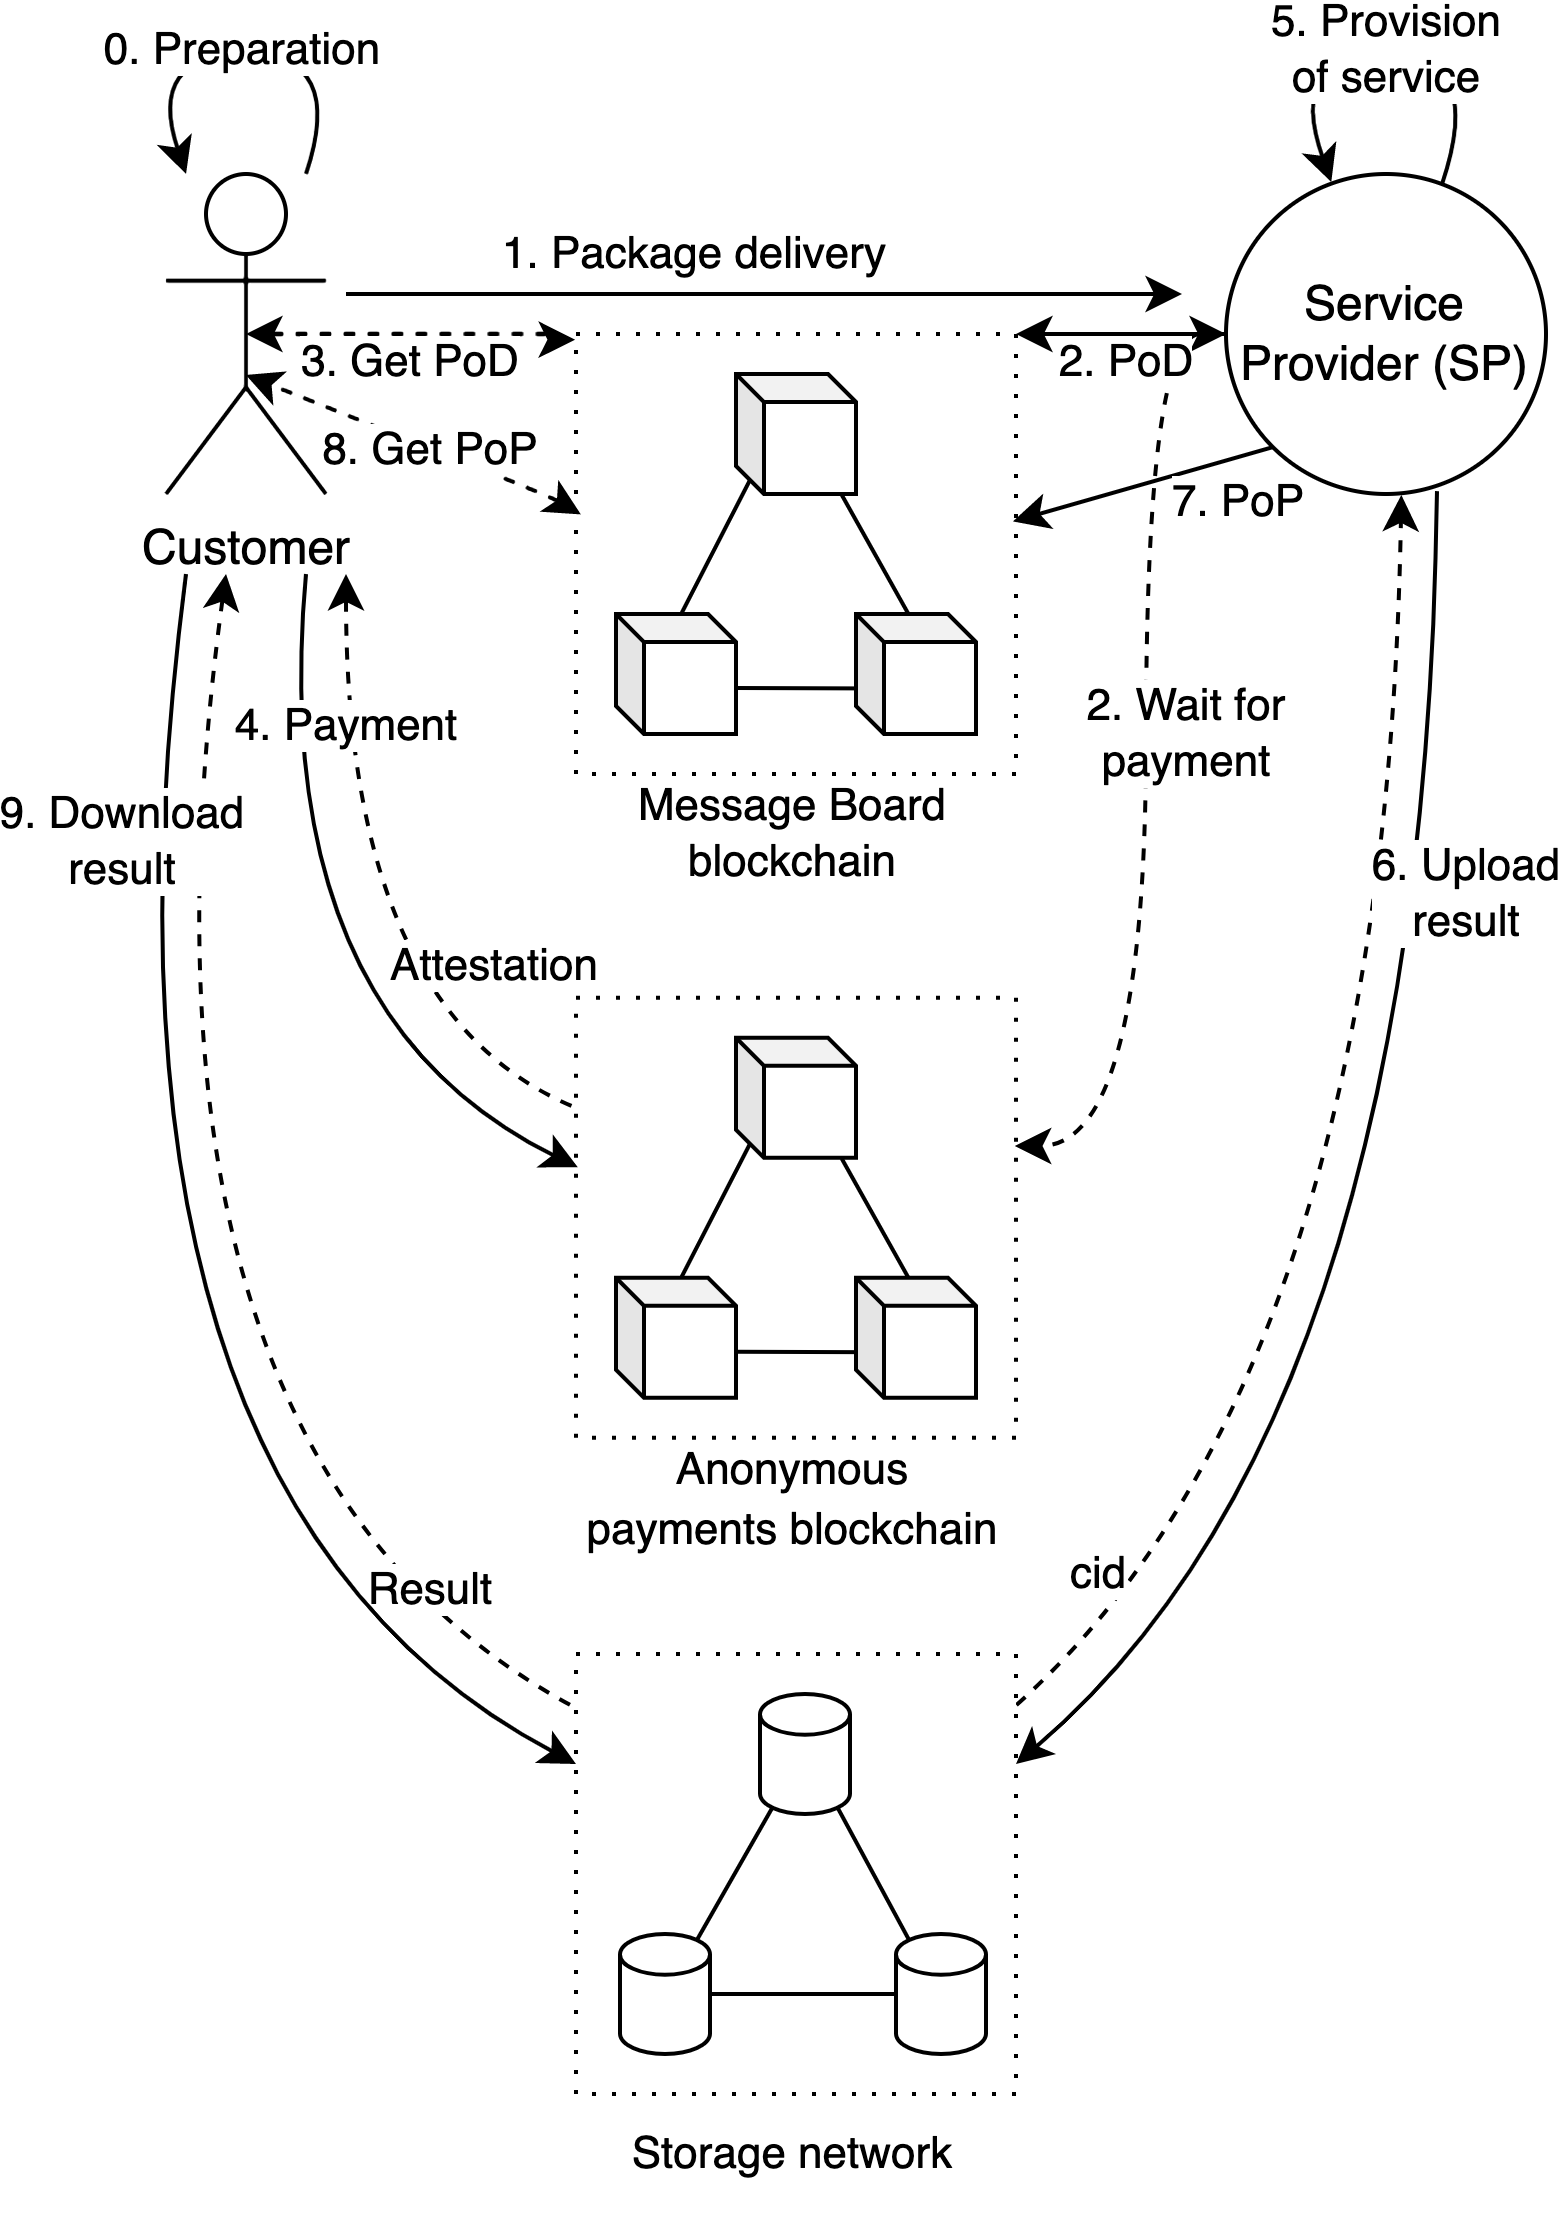
\includegraphics[width=\linewidth]{anonser-protocol.png}
\centering
\caption{Messages exchanged in the protocol.}
\label{fig:protocol-diagram}
\end{figure}

\noindent \textbf
{Step 0.  Preparation}\label{step-0-preparation}

The customer collects all the $\mathrm{materials}$ required by the SP, generates a random $\mathrm{provisionID}$ and a random keypair $(\mathrm{sk(C)},\mathrm{pk(C)})$. The $\mathrm{provisionID}$ will be used to associate all actions related to the transaction throughout the protocol. The $\mathrm{provisionID}$ and $\mathrm{pk(C)}$ are encoded as a QR code, printed, and sticked to the package $\mathrm{pkg}$. The $\mathrm{sk(C)}$ is kept secret and used to decrypt the $\mathrm{result}$ at the end of the protocol.

\noindent \textbf
{Step 1. Package delivery}\label{step-1-package-delivery}

The protocol starts once the customer delivers package $\mathrm{pkg}$ to the SP and its content gets accepted. As a result, $\mathrm{PoD}$ is created with predefined payment deadline $\mathrm{T}_\mathrm{pay}$, service provision deadline $\mathrm{T}_\mathrm{provide}$, and current time $\mathrm{T}_\mathrm{issue}$. Also $\mathrm{PoD}$ embodies the information whether the service has been paid in cash or should be paid by the customer using the anonymous blockchain account. In the latter case, the SP's payment $\mathrm{address}$ is included in the $\mathrm{PoD}$.

The digital signature $\mathrm{sig}_{\mathrm{sk}(\mathrm{SP})}$ on the $\mathrm{PoD}$ created with the SP's secret key $\mathrm{sk}(\mathrm{SP})$ guarantee non-repudiation.

Symbolically: 
\[
\mathrm{PoD \gets delivery(pkg)}
\]

\noindent \textbf
{Step 2. Proof of Delivery}\label{step-2-pod}

Then, the $\mathrm{PoD}$ is published on the message board by the SP, commiting to the fact that the package $\mathrm{pkg}$ has been delivered, adn the SP can not reject receiving it. If the provision has not been paid in cash, the SP waits for the customer to pay for the service on the specified in the $\mathrm{PoD}$ payment $\mathrm{address}$.

Symbolically: 
\[
\mathrm{publish(PoD)}
\]

\noindent \textbf
{Step 3. Get Proof of Delivery}\label{step-3-get-pod}

Once the package is delivered and the $\mathrm{PoD}$ is published, the customer can get the $\mathrm{PoD}$ from the message board and (if everything is correct) proceed with the protocol.

Symbolically: 
\[
\mathrm{PoD \gets get(provisionID)}
\]

\noindent \textbf
{Step 4. Payment}\label{step-4-payment}


If the provision has not been paid in cash, the customer should pay for the transaction with the predefined anonymous payment blockchain (see section~\ref{payment-for-services}).

In return, the customer receives the $\mathrm{attestation}$ that should be disclosed in case of a dispute.

Symbolically: 
\[
\mathrm{attestation \gets payment(address)}
\]

\noindent \textbf
{Step 5. Provision of service}\label{step-5-provision-of-service} 
Once the customer has paid for the transaction either in cash or using the anonymous blockchain, the SP can start providing the service.

Symbolically: 
\[
\mathrm{result \gets provision(materials)}
\]

\noindent \textbf
{Step 6. Upload result}\label{step-6-upload-result}

After the service is finished, a result should be created. 
Next, the result is encrypted using shared key derived from the customer's public key $\mathrm{pk(C)}$ and the SP's secret key $\mathrm{sk(S)}$ using Diffie-Hellman key exchange (DHKE) method.

The encrypted result is then uploaded on the content addressable network (such as IPFS). In return the content identifier ($\mathrm{cid}$) is created.

Symbolically: 
\[
\mathrm{cid \gets upload(E_{DHKE(sk(SP), pk(C))}(result))}
\]

\noindent \textbf
{Step 7. Proof of provision}\label{step-7-proof-of-provision}

When the $\mathrm{result}$ is uploaded, the SP creates and publish on a message board a proof of provision consisting of $\mathrm{cid}$ along with $\mathrm{provisionID}$ and signature $\mathrm{sig}_\mathrm{SP}$.

Symbolically: 
\[
\mathrm{publish(PoP)}
\]

\noindent \textbf
{Step 8. Get Proof of Provision}\label{step-8-get-proof-of-provision}

After delivering the package and paying for the transaction, the customer start listening to the message board and waits until the SP publishes the $\mathrm{PoP}$ for the $\mathrm{provisionID}$.

Symbolically: 
\[
\mathrm{cid \gets get(provisionID)}
\]

\noindent \textbf
{Step 9. Download result}\label{step-9-download-result} 
Having the $\mathrm{cid}$, the customer downloads and decrypts the $\mathrm{result}$ using shared key derived from the customer's secret key $\mathrm{sk(C)}$ and the SP's public key $\mathrm{pk(S)}$ using DHKE method. The protocol ends.

Symbolically: 
\[
\mathrm{result \gets D_{DHKE(sk(C), pk(SP))}(download(cid))}
\]

\section{Fairness analysis}\label{sec:fairness-analysis}
We analyze the fairness of the protocol by representing it as an interactive non-cooperative game.

\subsection{Model}\label{sec:fairness-model}
We consider three positions:

\begin{itemize}
\item Neutral position (•): when a party has not spent nor gained anything of significant value (money, time, effort). For example, at the beginning of the protocol.
\item Disadvantaged position (-): when a party has put a significant value without receiving an equivalent. For example, the customer has paid for a service in advance.
\item Advantaged position (+): when a party would benefit if the transaction would halt at that step. For example, the SP has received payment before service provision.
\end{itemize}

There are many actions that each party can take, but we group them into two categories:

\begin{enumerate}
\def\labelenumi{\arabic{enumi}.}

\item Normal: taking actions prescribed by the protocol.
\item Abnormal: everything that deviates from the designed steps of the protocol. For example, sending an arbitrary message, skipping or repeating steps, timing out.
\end{enumerate}

Moreover, at any step of the protocol, the customer can start a dispute; therefore, another dimension with two positions has to be considered:

\begin{enumerate}
\def\labelenumi{\arabic{enumi}.}

\item Agree: the customer agrees with the action and therefore does not start a dispute.
\item Start a dispute: the customer disagrees with the action and therefore starts a dispute.
\end{enumerate}

As a result, in our analysis, we have to consider four different outcomes for each party of the protocol ($\mathrm{party \in \{c, s}\}$), for each step of the protocol ($\mathrm{step \in 1..9}$):

\begin{itemize}

\item
  $\mathrm{\sigma_{step,party,n}}$: after following the protocol when the other party acted normally.
\item
  $\mathrm{\sigma_{step,party,d}}$: after a settled dispute when the other party acted normally.
\item
  $\mathrm{\sigma_{step,party,\overline{n}}}$: after not starting a dispute despite the other party has acted abnormally.
\item
  $\mathrm{\sigma_{step,party,\overline{d}}}$: after a settled dispute when the other party has acted abnormally.
\end{itemize}



The protocol terminates after the last step, after starting a dispute, or after a party has not completed its designated action in time. Therefore, all positions except $\mathrm{\sigma_n}$ are termination positions.

Because the customer is anonymous, the SP can not start a dispute—there is no means to identify the customer. To mitigate the issue, we designed the protocol so that the SP who follows the protocol is always in an advantaged position, and therefore has no reason to start a dispute. On the other hand, the customer can start a dispute at any time of the protocol, but only the actual misbehaviour of the SP makes him win the case.

\begin{definition}[Fairness] \label{def:fairness}
A protocol achieve fariness iff 
\begin{equation*}
\begin{split}
\forall_{party \in parties}\forall_{\mathrm{step} \in \mathrm{steps}} &\operatorname{can\ move}\\
&\operatorname{to\ the\ non-disadvantaged\ position} 
\end{split}
\end{equation*}

\end{definition}


\subsection{Assumptions}\label{assumptions}

Below we listed assumptions we took for the analysis purpose.  

\begin{itemize}

\item
    Both parties start from a neutral position (•).
\item
    After completing a transaction, both parties end up in advantaged positions (+). In other words, they have intrinsic motivation to initialize and complete the transaction.
\item
    The protocol steps are atomic—there are no intermediate steps.
\item 
    The protocol can go only forward—there is no way of reverting any action.
\item
    Repeating the first step starts a new transaction. Repeating any other step is considered abnormal and gets ignored. For example, paying for the invoice twice does not cause any effect on the curse of the protocol.
\item 
    Once published, the result is available to the customer on the storage network. The idea of guaranteeing it cryptographically is discussed in section~\ref{sec:discussion}.
    
\item
    Winning the dispute leads to a neutral position (•).

\item
    Losing the dispute leads to a punishment greater than any reward, leading to a disadvantaged position (-). Hence, the rational customer will not start a dispute that he is unsure of winning.
\item
    Both the customer and the SP are rational (selfish). They always prefer to go from the worst position to a better position, but also risk a temporary worst position in favour of a later better position if and only if it is assured that they will not be stuck in the worst position.
\end{itemize}

\subsection{Steps}\label{sec:steps}

Figure~\ref{fig:positions} shows the positions of each party after each possible action taken.

\begin{figure}[h!]
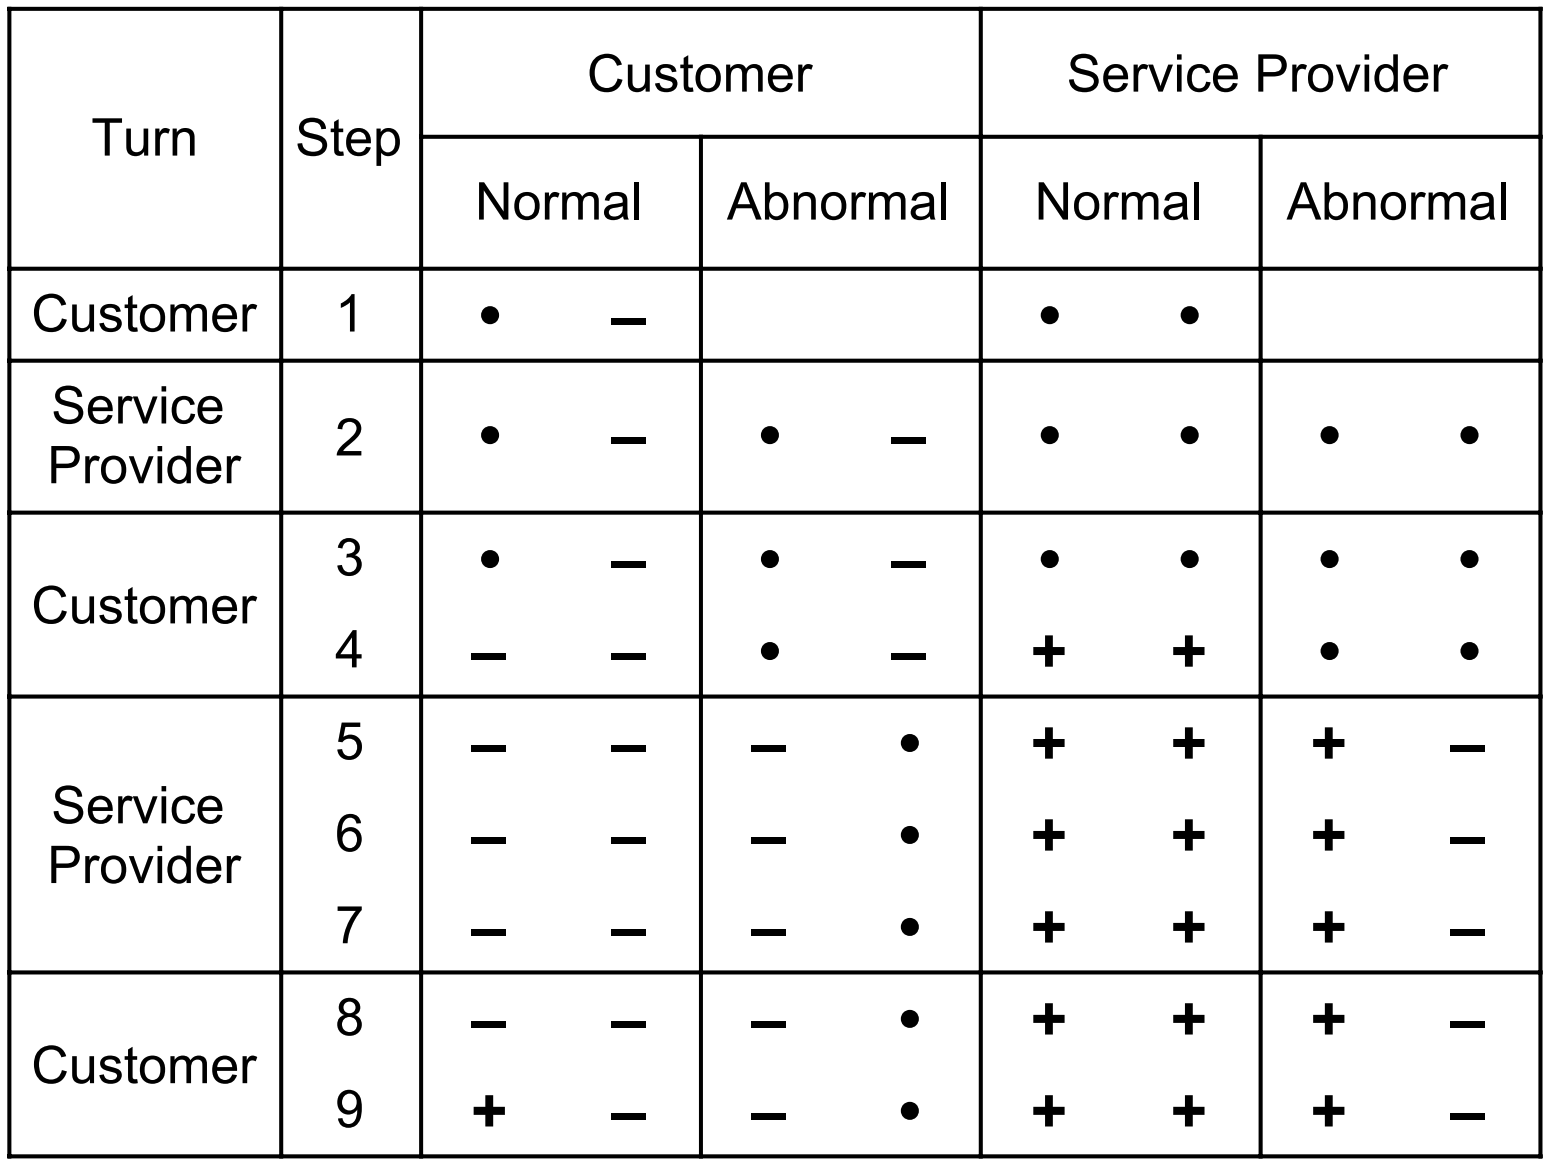
\includegraphics[width=9cm]{formal-table-of-positions.png}
\centering
\caption{Positions after each step of protocol}
\label{fig:positions}
\end{figure}

The description of each step and the rationale of the outcome position is given in the Appendix~\ref{app:proof-of-fairness}.

\subsection{Example scenarios}\label{example-scenarios}

The figure~\ref{fig:misbehaviour} shows the transitions of positions when the SP tries to misbehave and does not execute service after receiving the payment. The customer reacts by starting a dispute and the protocol ends up neutral to the customer and disadvantaged to the SP positions.

\begin{figure}[h!]
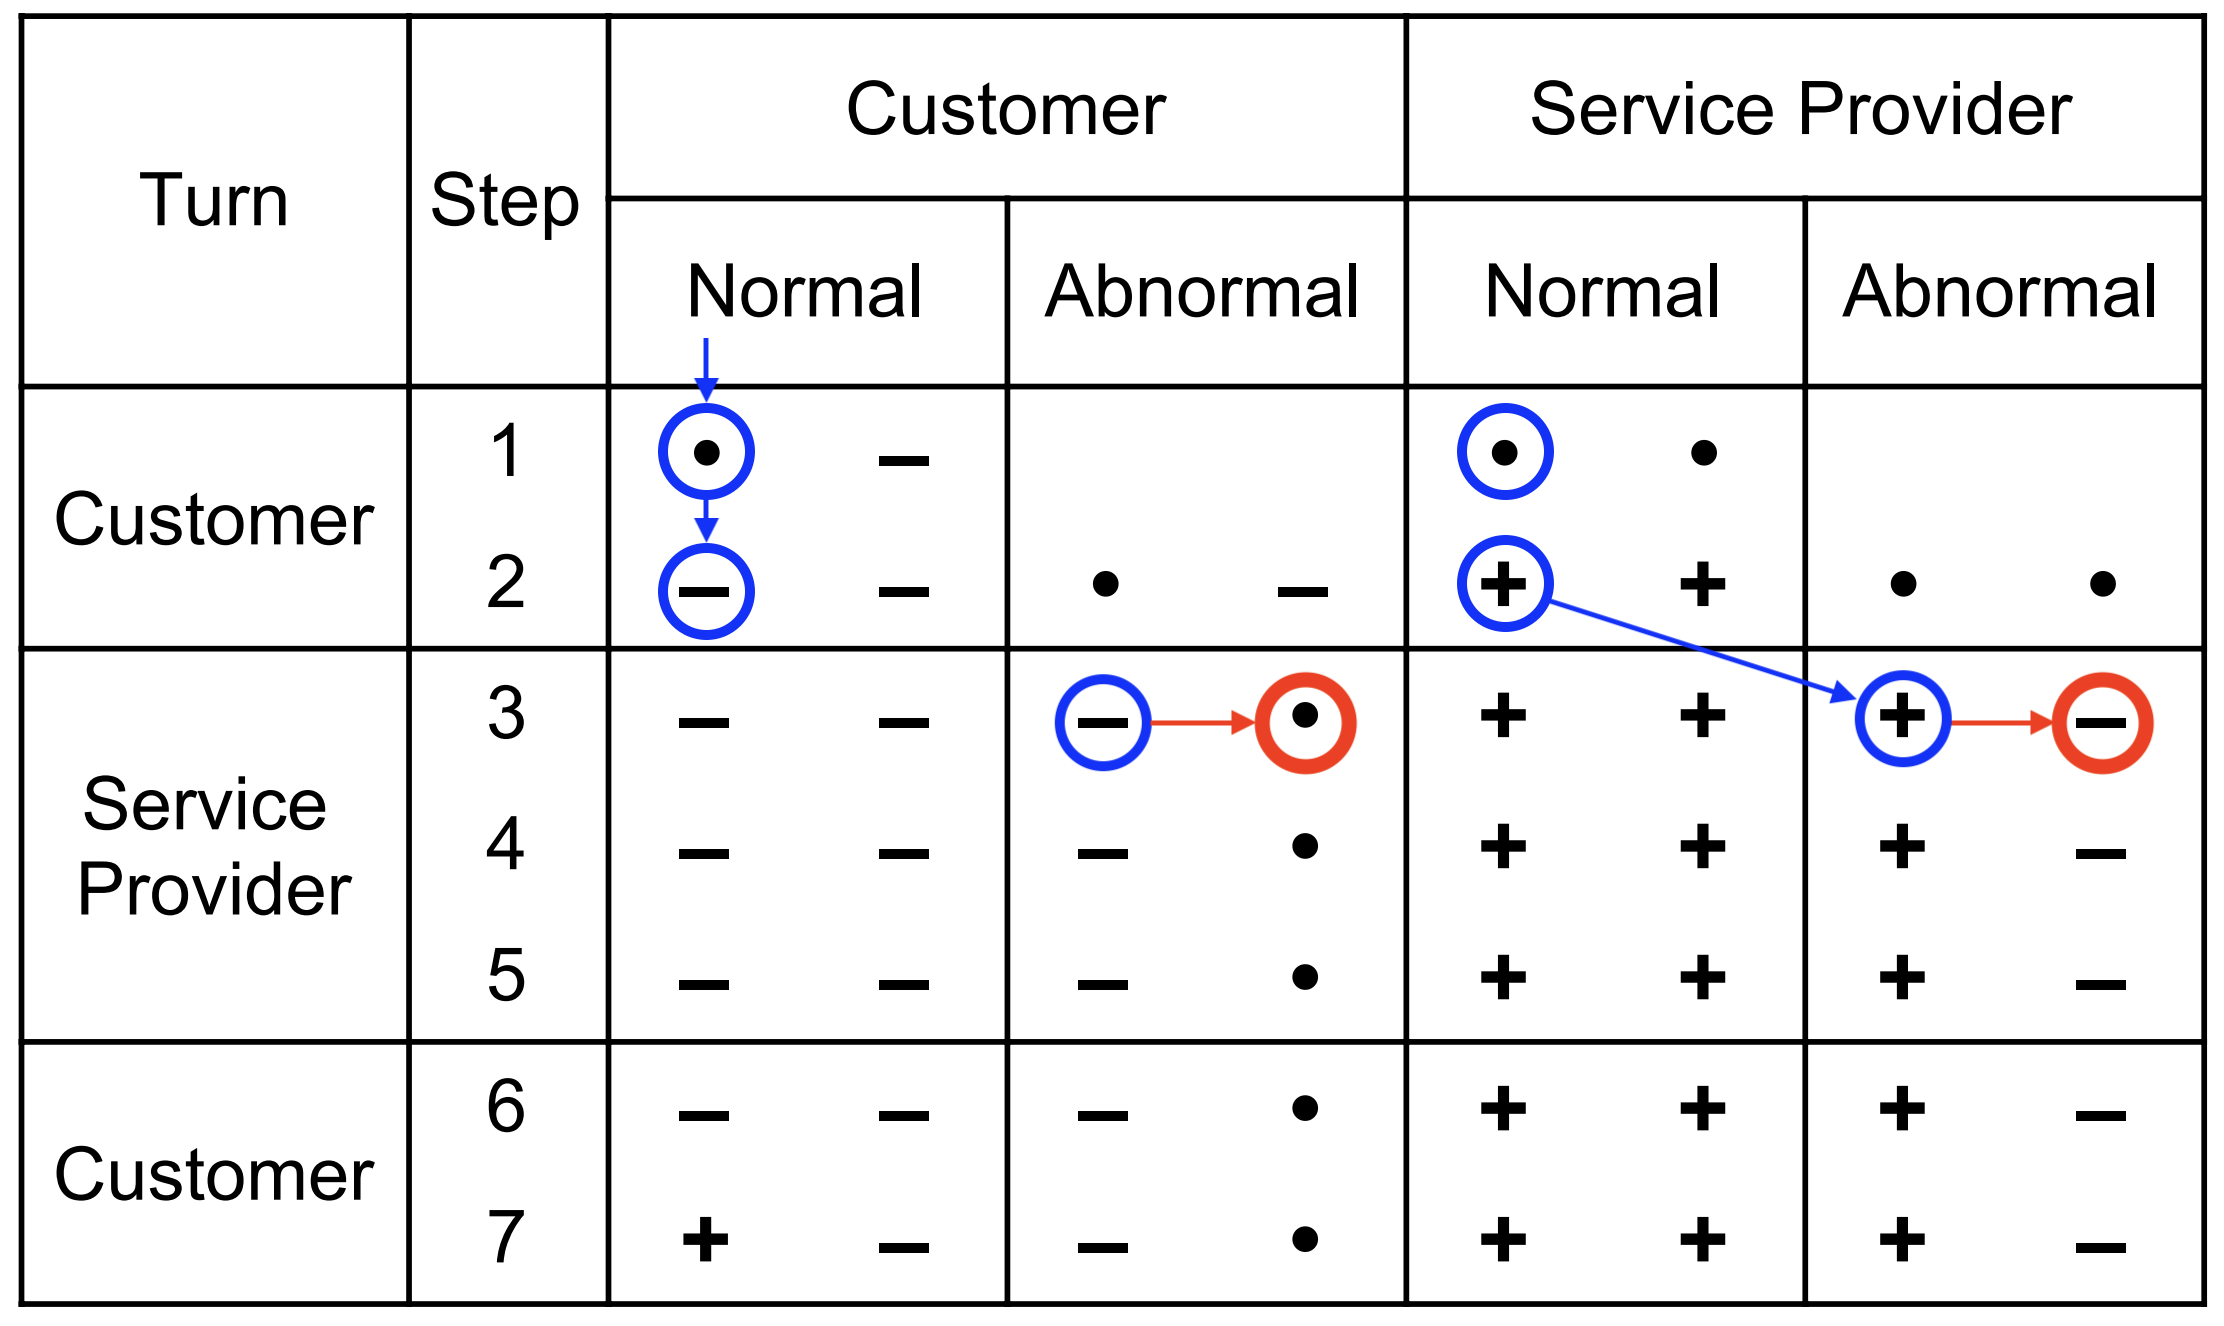
\includegraphics[width=9cm]{formal-misbehaviour-path.png}
\centering
\caption{Transitions of positions where the SP is misbehaving and the customer starts a dispute}
\label{fig:misbehaviour}
\end{figure}

Ultimately, the rational path for both parties is to follow the protocol as shown in the figure~\ref{fig:rational}.

\begin{figure}[h!]
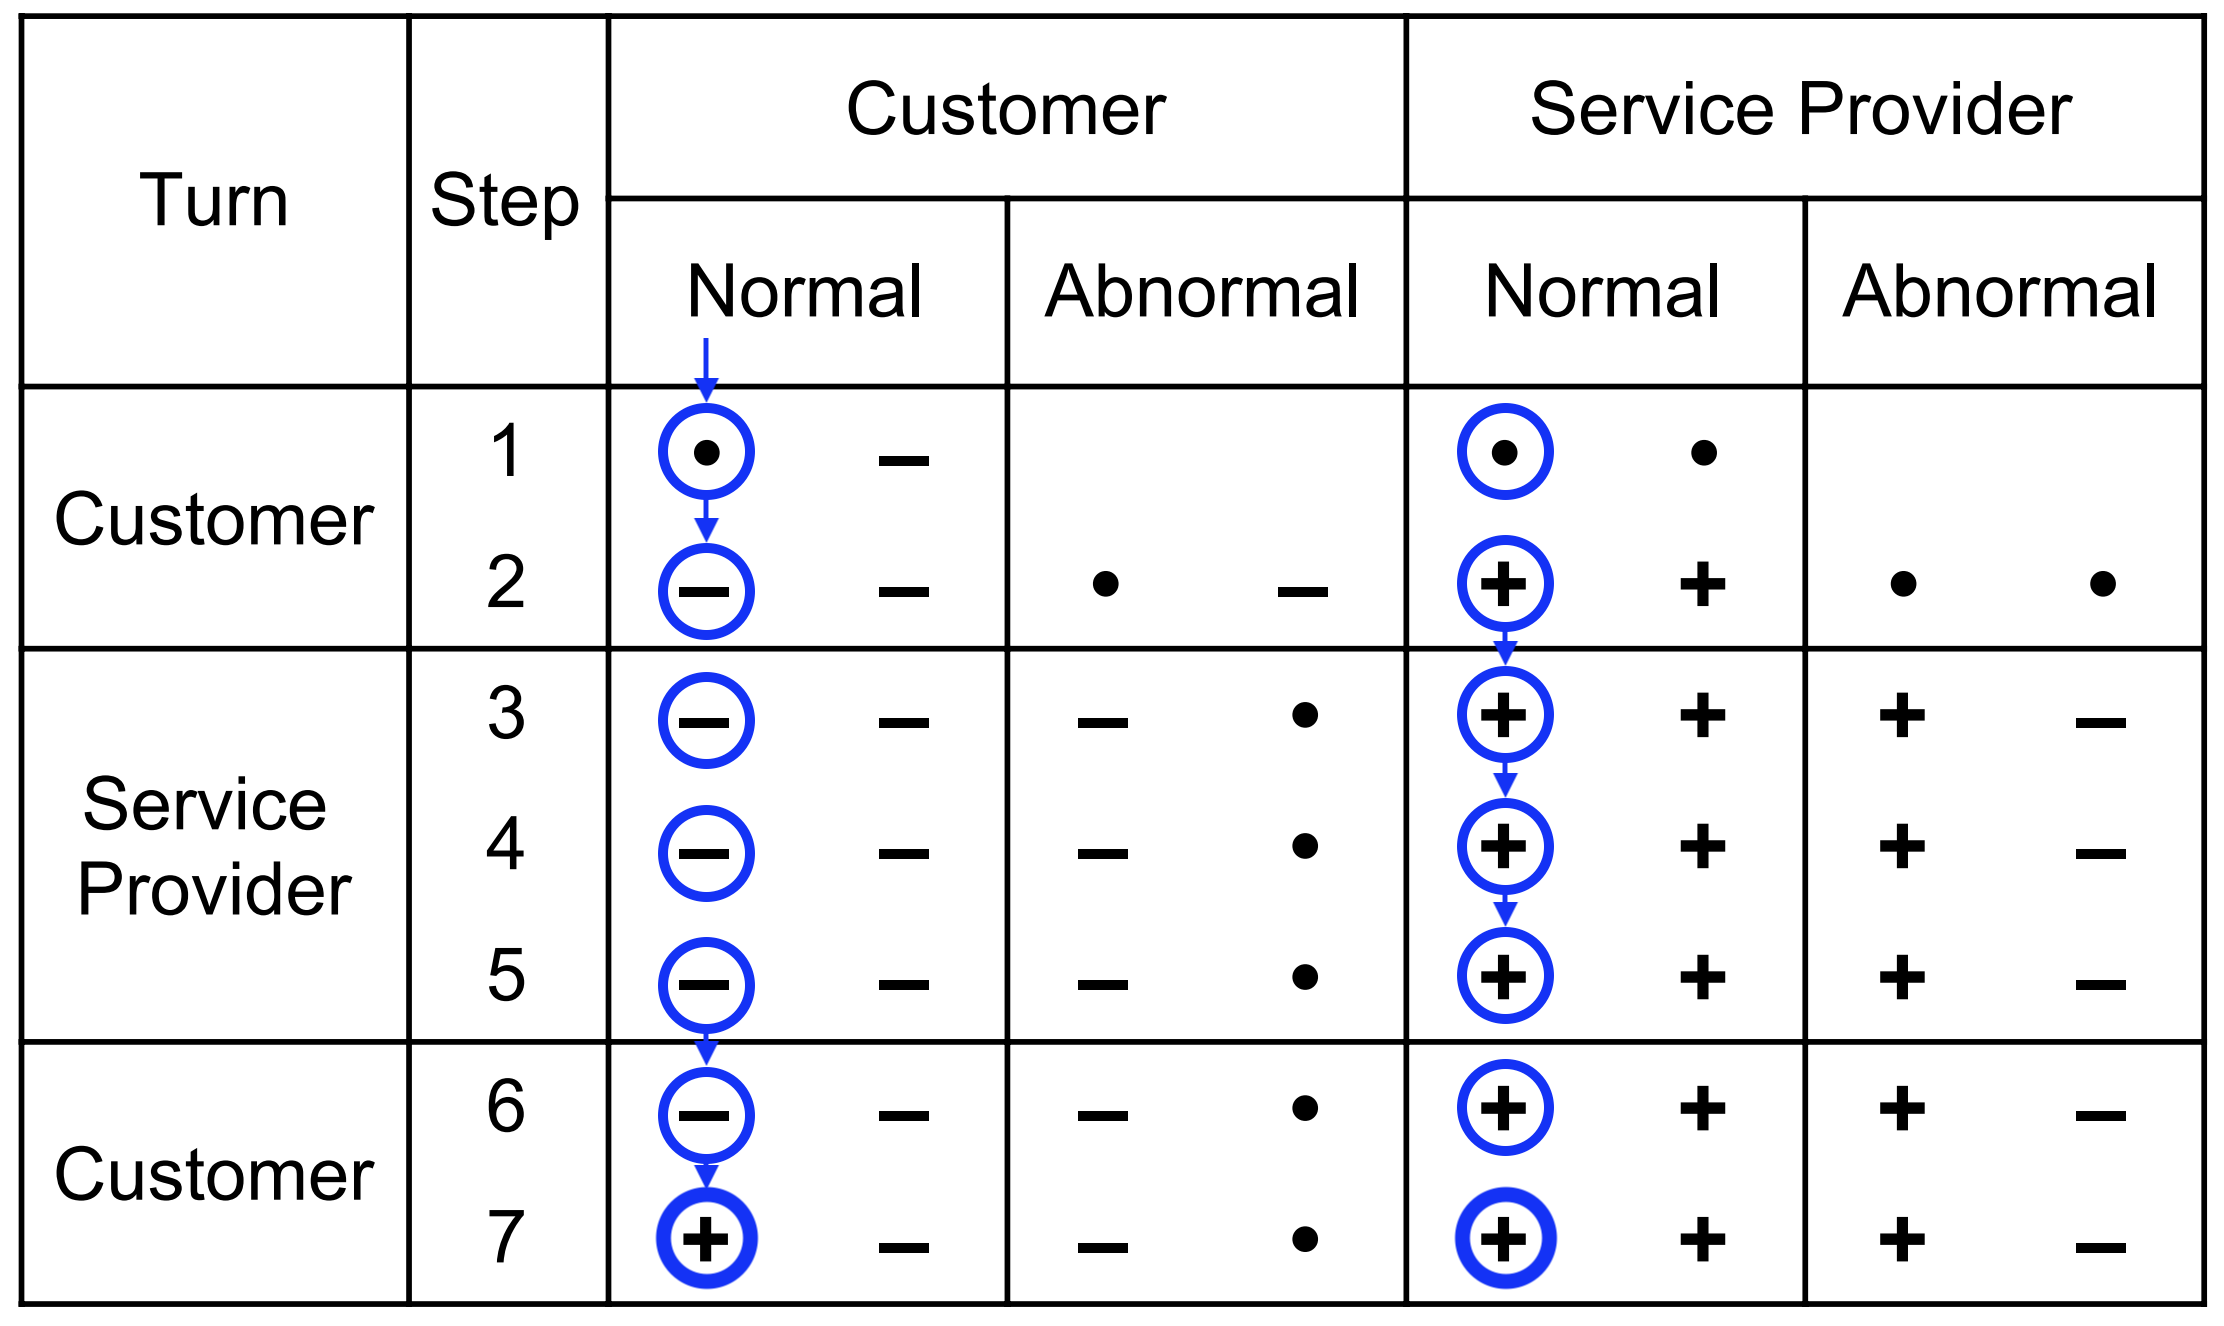
\includegraphics[width=9cm]{formal-rational-path.png}
\centering
\caption{Transitions of positions where where both the customer and the SP are behaving correctly}
\label{fig:rational}
\end{figure}

Using the fariness definition~\ref{def:fairness} and the assumptions stated in section~\ref{assumptions}, our analysis indicates that the protocol achieves fairness.

\section{Experiments}\label{sec:experiments}

\subsection*{Setup}

We have developed a prototype of our protocol using the following technologies:

\begin{itemize}
  \item{Anonymous payments} — we use the Monero blockchain \cite{noetherRingSignatureConfidential2015}.
  \item{Storage netowork} — we use the Powergate\footnote{https://github.com/textileio/powergate}, which is a wrapper around Filecoin and IPFS.
  \item{Message board} — we use the Ethereum blockchain \cite{woodEthereumSecureDecentralised2014}; concretely, Truffle Ganache\footnote{https://trufflesuite.com/ganache/} and Solidity language.
  \item{Customer and SP} — we create client side web application (webapp) using \texttt{React}\footnote{https://reactjs.org} for creating UI, \texttt{web3.js}\footnote{https://web3js.org} for interaction with Ethereum, and \texttt{crypto-js}\footnote{https://github.com/brix/crypto-js} for encryption. We use \texttt{MetaMask}\footnote{https://metamask.io} browser extension for signing and submiting transactions to Ethereum's node. We use \texttt{monerod}\footnote{https://monerodocs.org/interacting/monerod-reference/} network client and \texttt{monero-wallet-cli}\footnote{https://monerodocs.org/interacting/monero-wallet-cli-reference/} command-line interface for interacting with Monero blockchain.
\end{itemize}

The prototype is available at \url{https://anonser.stan.bar}. The source code is available at \url{https://github.com/stanbar/anonymous-provision-of-services-via-blockchain}.

We developed and tested our prototype in the following environment:

\begin{itemize}
  \item{OS} — Arch Linux 5.11.8
  \item{Docker} — 20.10.5
  \item{CPU} — Intel(R) Core(TM) i7-4790 (8) 4.00~GHz
  \item{RAM} — 16 GB DDR3
  \item{Storage} — Samsung PM85 256~GB SSD

  \item{monerod and monero-wallet-cli} — v0.18.1.2
  \item{Powergate} — v2.6.2
  \item{Ganache} — v7.5.0
  \item{Solidity} — v0.8.17
  \item{ReactJS} — v18.0.25
  \item{web3.js} — v1.8.1
  \item{crypto-js} — v4.1.1
\end{itemize}

For simplicity, all components run on one, mentioned above, physical machine; and all processes are managed by Docker. 

Moreover, Powergate is configured to use local Filecoin and IPFS networks.
For Ethereum blockchain we use Truffle Ganache, which is a local Ethereum blockchain for development and testing purposes. 
Monero is configured to use the public stage network.
We assume service provider offers only one type of service, which is offered for a fixed public price, hence we omit the type of service and price from the protocol.

\subsection*{Preparation}

Both the customer and the SP create a Monero wallets using \texttt{monero-wallet-cli} command-line tool.

Service provider deploys the smart contract using the \texttt{truffle migrate --network development} command, which deploys the smart contract to the Ethereum blockchain. The webapp is configured to use the latest deployed smart contract address.

Customer gets some testing Monero funds using \url{https://community.rino.io/faucet/stagenet/} faucet service.

Next, the customer enable per-transaction proof generation (payment \texttt{attestation}) by setting \texttt{set store-tx-info 1} for his wallet. The proof generation is required to verify the payment in case of dispute.

At this point both the customer and the SP are ready to start the protocol.

\subsection*{Experiment}

The customer and the SP are two different users of our prototype, but for simplicity they use the same machine and the same web application.

Now we describe the experiments we performed to test our protocol.


\begin{figure*}[ht]
  \begin{center}
  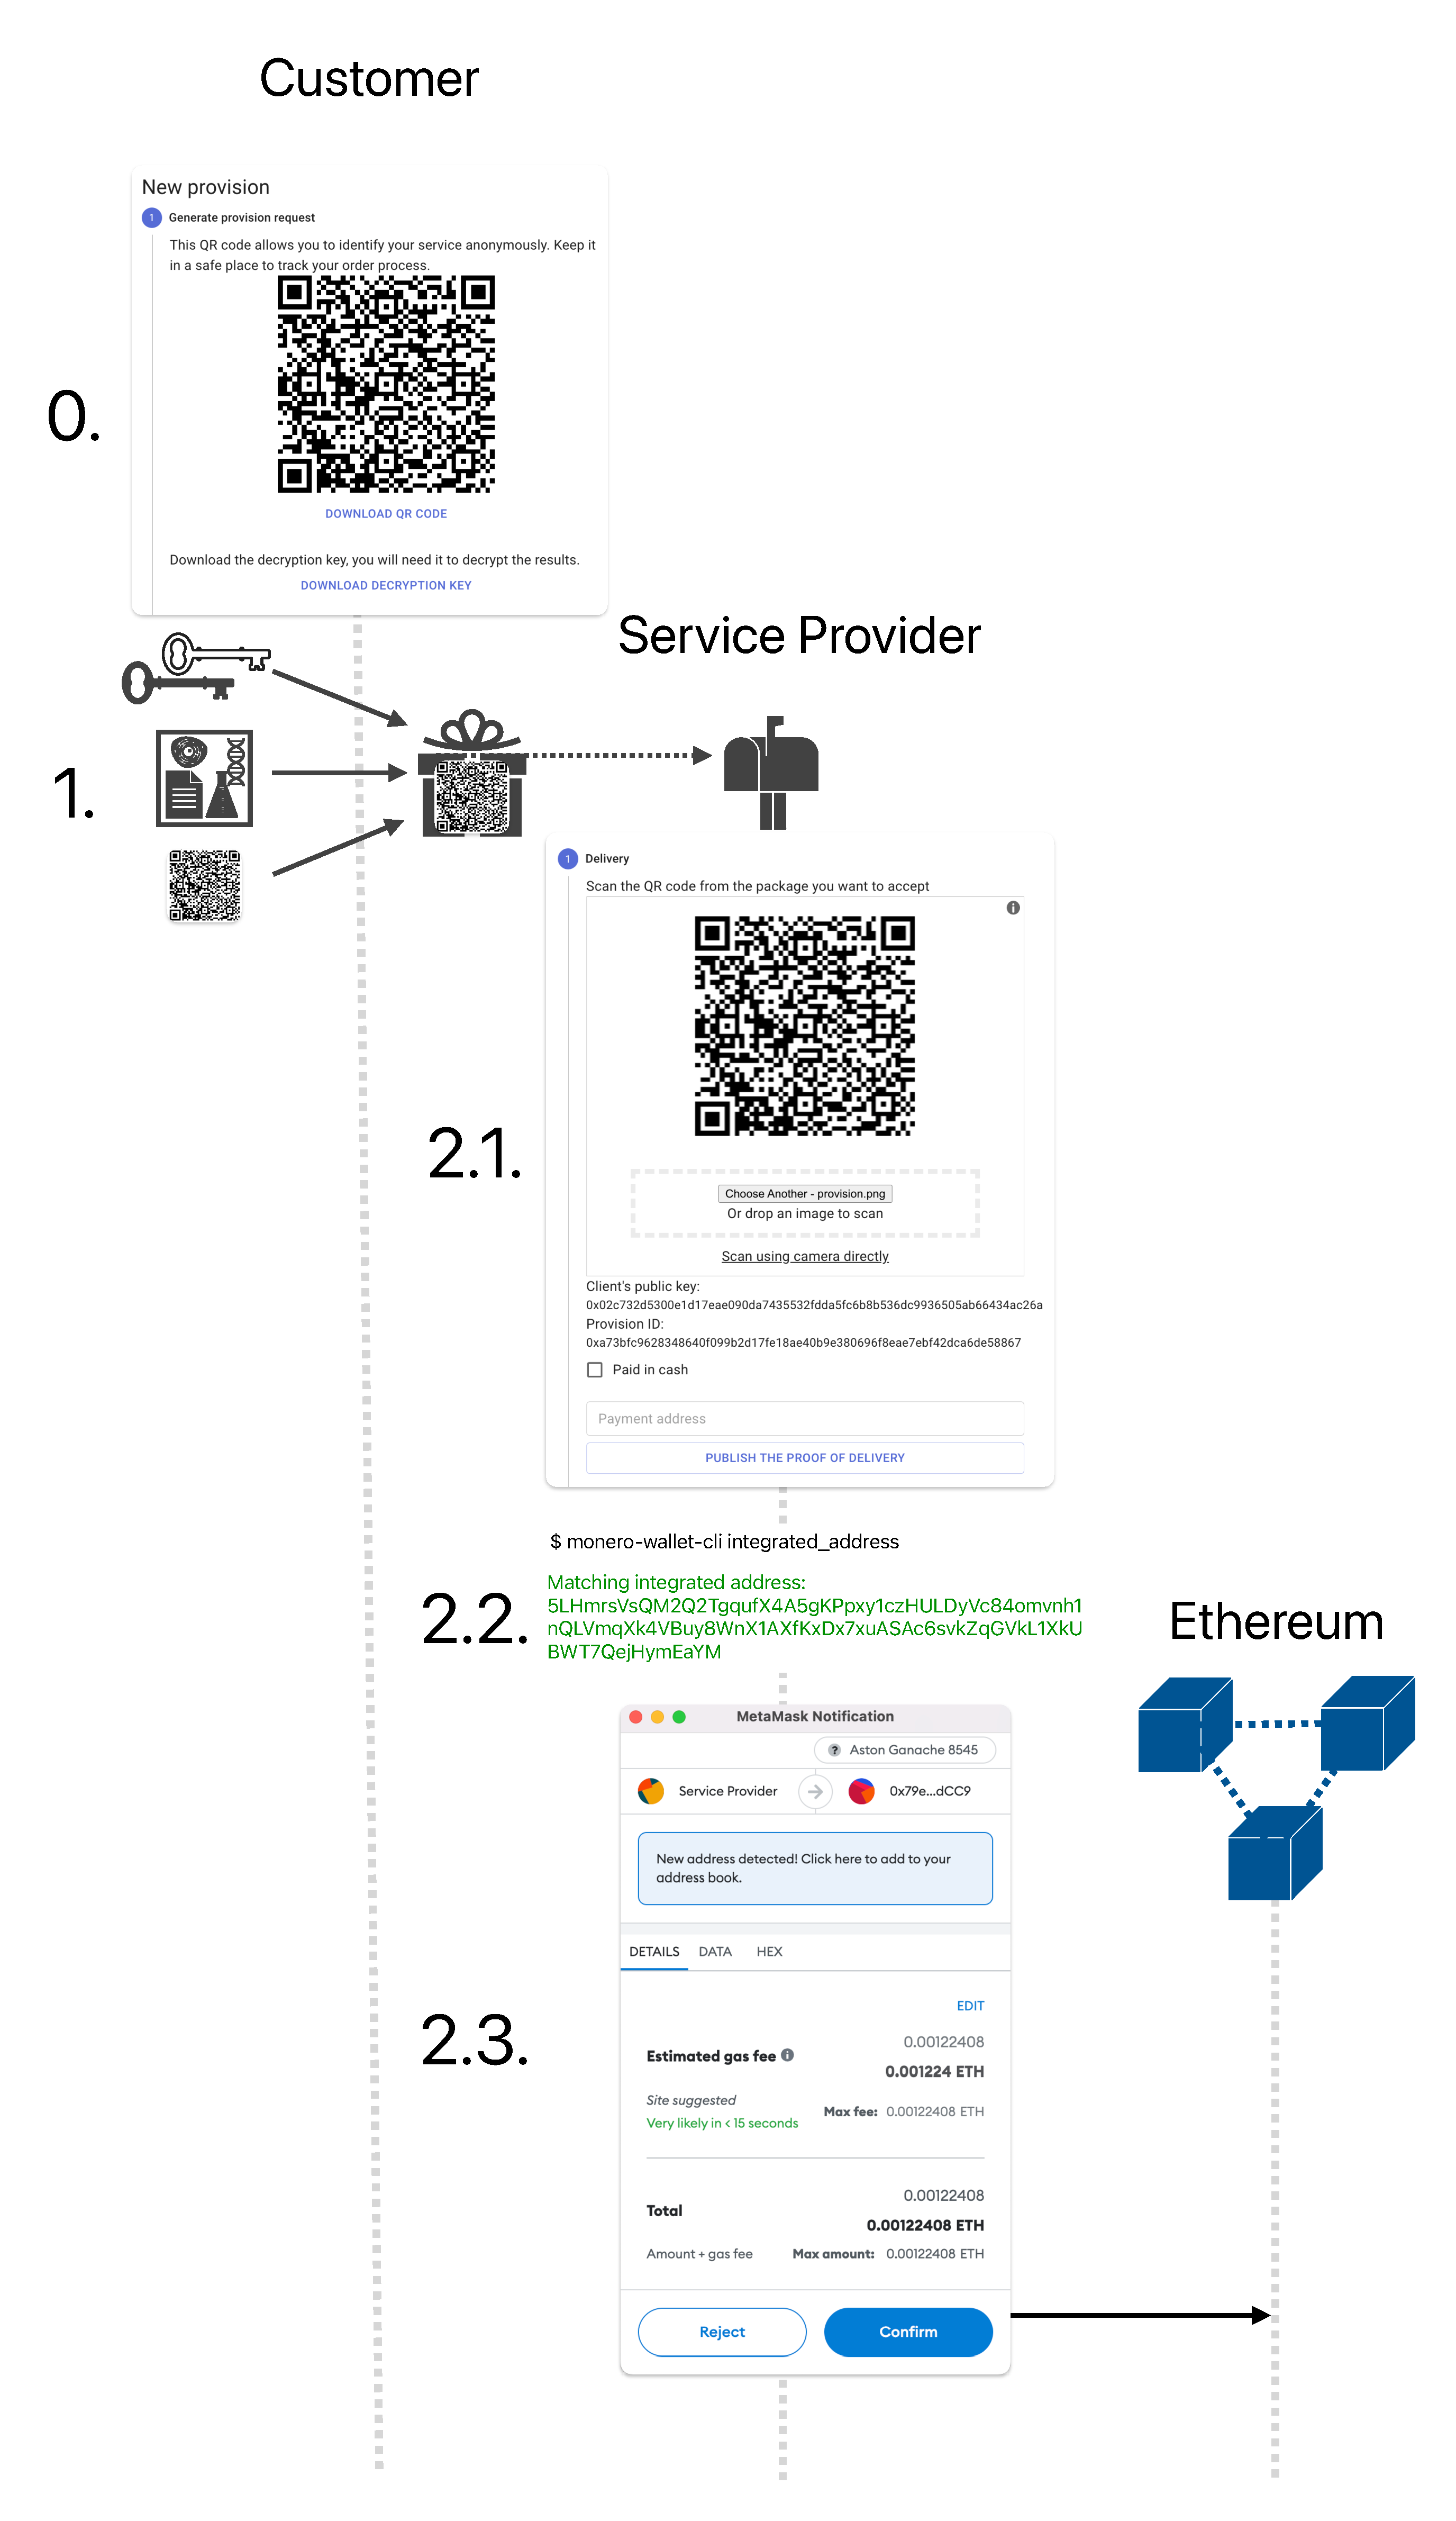
\includegraphics[width=\textwidth,height=\textheight,keepaspectratio]{anonser-experiment1.pdf}
  \end{center}
\end{figure*}
\begin{figure*}[ht]
  \begin{center}
  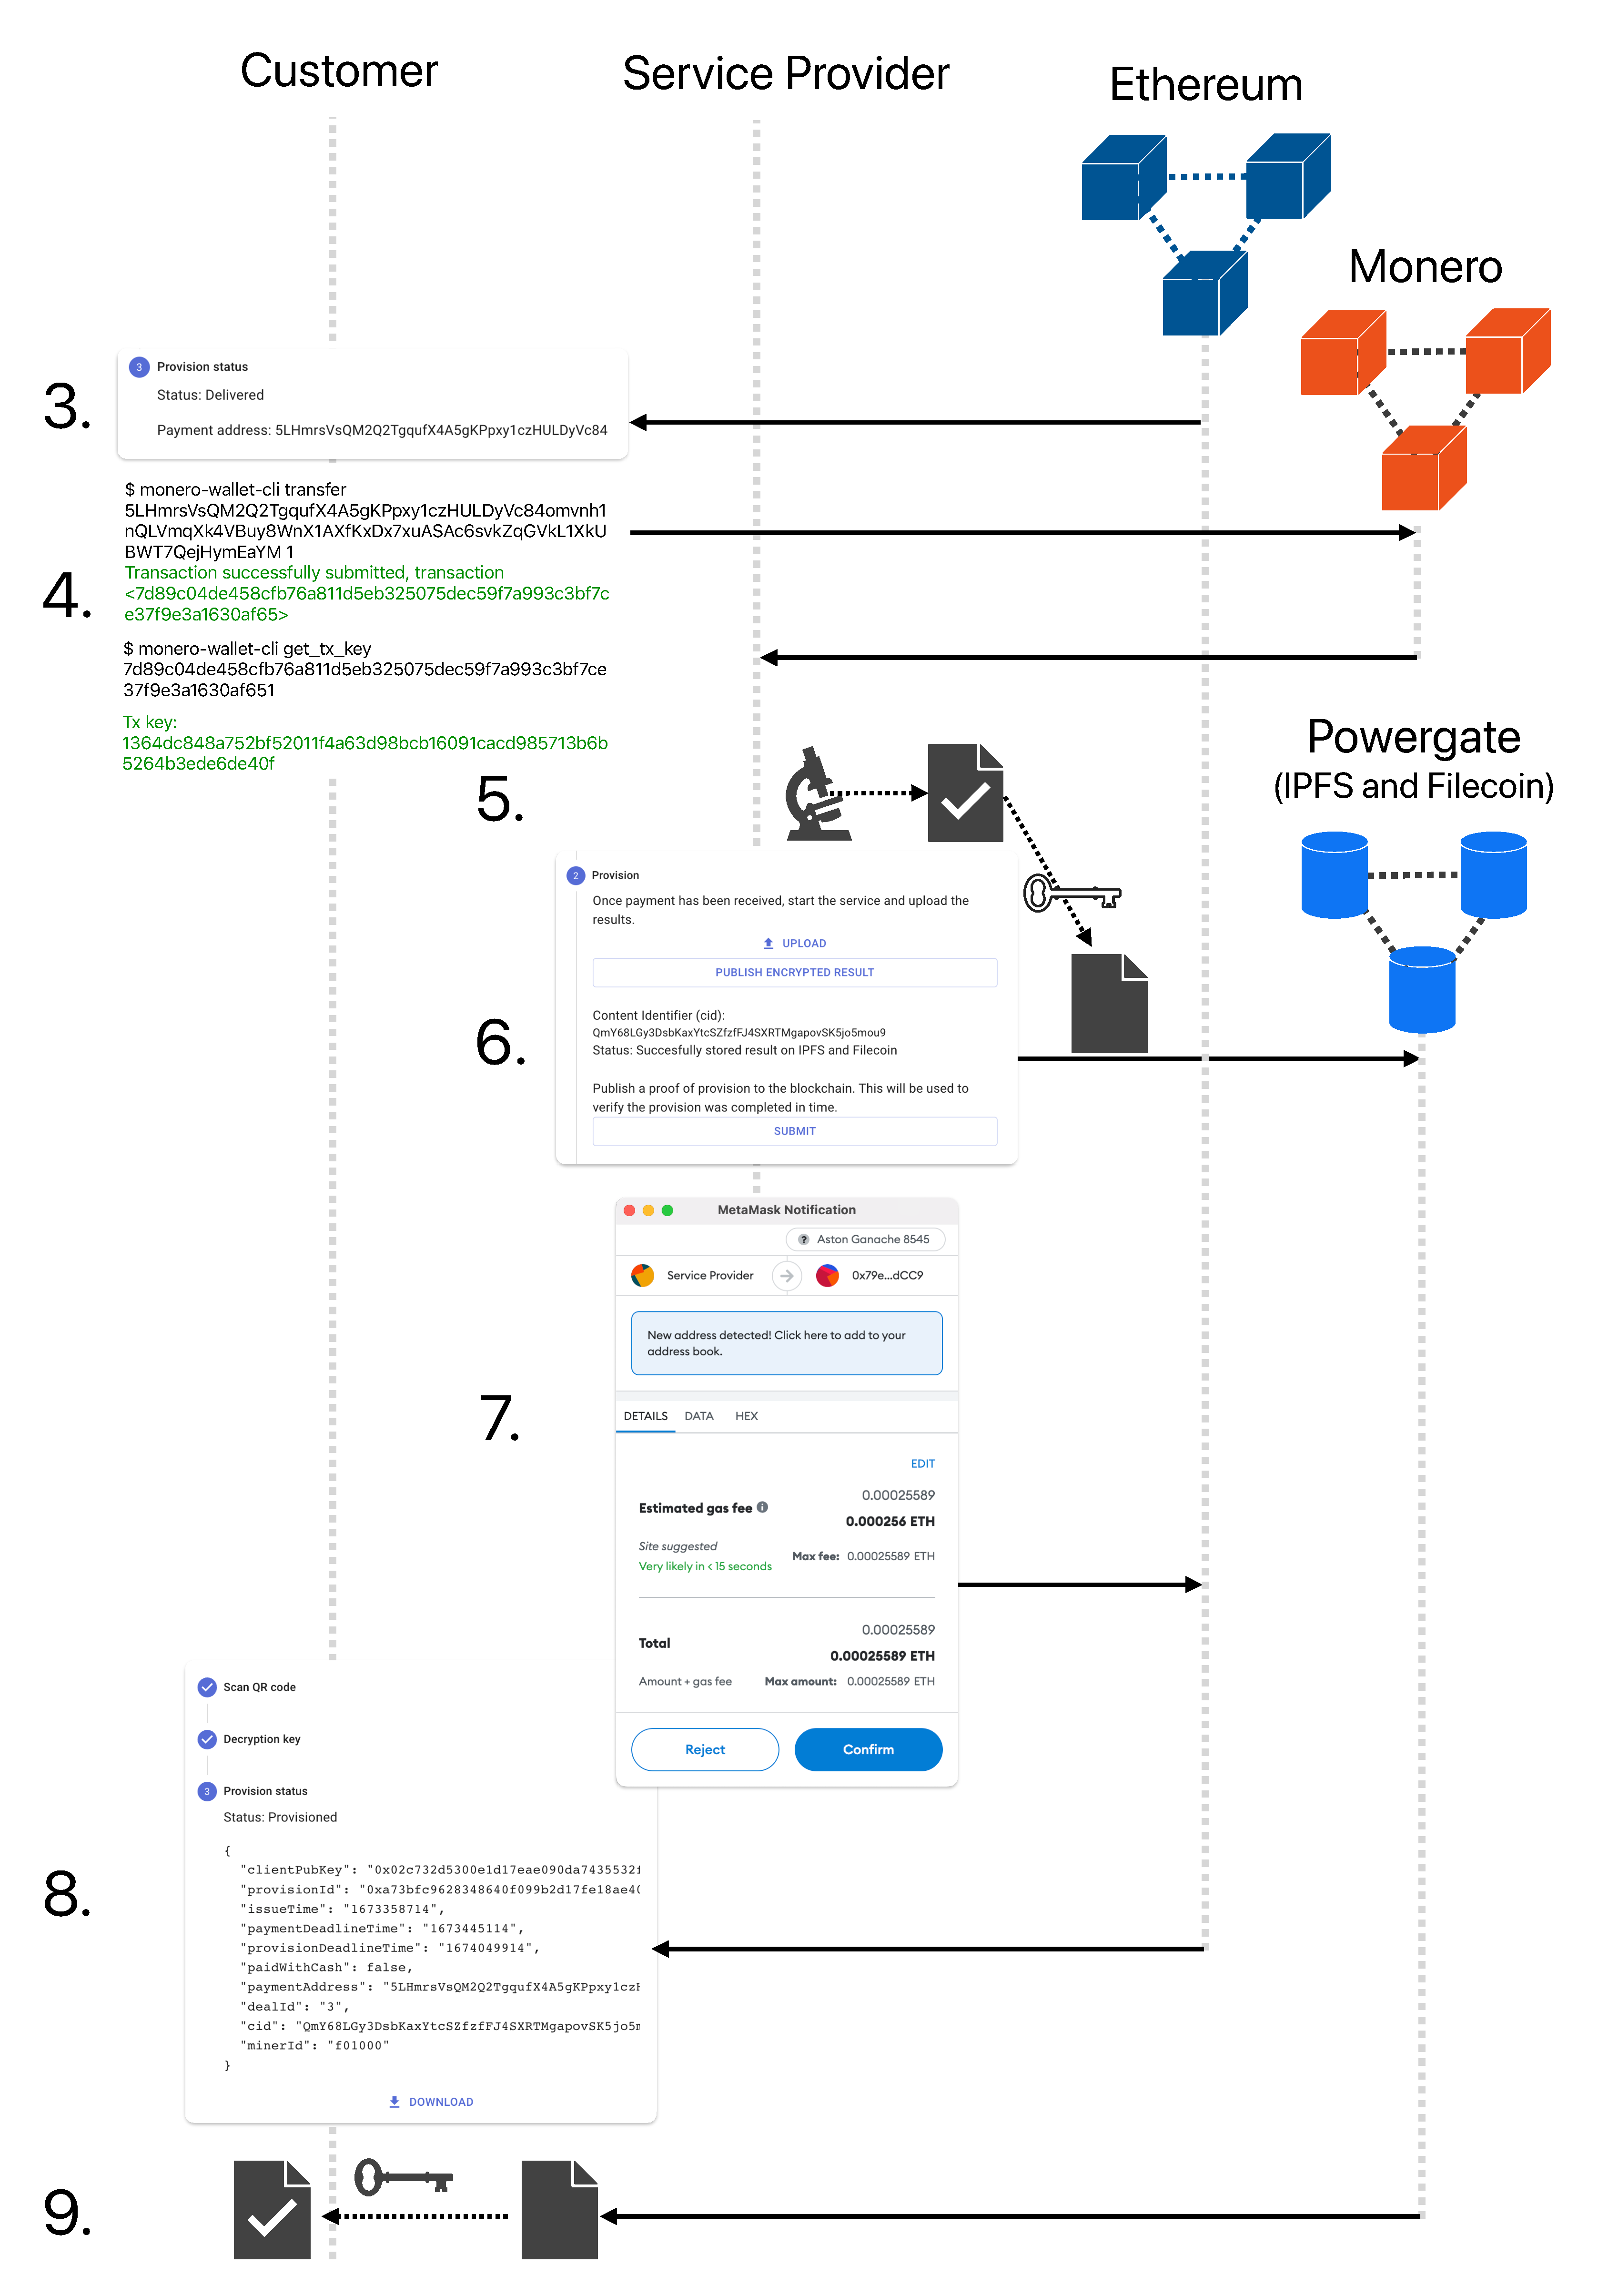
\includegraphics[width=\textwidth,height=\textheight,keepaspectratio]{anonser-experiment2.pdf}
  \end{center}
\end{figure*}

\begin{enumerate}
  \setcounter{enumi}{0}
  \item[0.] The protocol starts with the customer opening the webapp and creating new provision. 
The app generates random ECDSA (secp256k1) customer's keypair and random 32 bytes provisionID, then display QR code that encodes both the provisionID and the customer's public key. 
The customer's private key must be downloaded and provided later for the decryption of the results.

  \item[1.] The customer prints the QR code, stick it on a package, and delivers the package to the SP either: in person, via trusted party, or delivery agency.

  \item[2.1.] The SP opens the app, scans the QR code decoding the provisionID and the client's public key.

  \item[2.2.] Since (in this experiment) the provision has not been paid in cash, the SP generate unique Monero payment address using \texttt{monero-wallet-cli integrated\_address} 
  \item[2.3.] The SP submits the proof of delivery to the Ethereum blockchain using MetaMask interface. 

  % monero-wallet-cli --stagenet --wallet-file sp --password "" integrated_address
  % Random payment ID: <2b6d65d7d48b7896>
  % Matching integrated address: 5LHmrsVsQM2Q2TgqufX4A5gKPpxy1czHULDyVc84omvnh1nQLVmqXk4VBuy8WnX1AXfKxDx7xuASAc6svkZqGVkL1XkUBWT7QejHymEaYM
  \item[3.] The customer (using the webapp) check the transaction status on the Ethereum blockchain invoking \texttt{getProvision} with arguments \texttt{customerPubKey} and \texttt{provisionID}.
  % monero-wallet-cli --stagenet --wallet-file customer --password "" transfer 5LHmrsVsQM2Q2TgqufX4A5gKPpxy1czHULDyVc84omvnh1nQLVmqXk4VBuy8WnX1AXfKxDx7xuASAc6svkZqGVkL1XkUBWT7QejHymEaYM 1
  % Transaction successfully submitted, transaction <7d89c04de458cfb76a811d5eb325075dec59f7a993c3bf7ce37f9e3a1630af65>
  % monero-wallet-cli --stagenet --wallet-file customer --password "" get_tx_key 7d89c04de458cfb76a811d5eb325075dec59f7a993c3bf7ce37f9e3a1630af65
  % Tx key: 1364dc848a752bf52011f4a63d98bcb16091cacd985713b6b5264b3ede6de40f

  \item[4.] The customer (using the \texttt{monero-wallet-cli transfer}) sends the payment to the designated in the smart contract \texttt{paymentAddress} and stores the payment attestation (using \texttt{monero-wallet-cli get\_tex\_key <tx-id>}) in case of dispute.

  \item[5.] Once SP notice the payment on Monero blockchain it starts providing the service and outputs the file \texttt{result.pdf}.

  \item[6.] The SP uploads the file \texttt{result.pdf} on the Filecoin and IPFS networks using Powergate. In result, the SP gets the content identifier \texttt{cid}, and \texttt{dealID} and \texttt{minerID}.

  \item[7.] The SP submits a Proof of Provision transaction to the Ethereum blockchain by invoking \texttt{proofOfProvision} with arguments \texttt{customer\-PubKey}, \texttt{provisionID}, \texttt{cid}, and \texttt{dealID}.

  \item[8.] Meantime, the Customer subscribes to the Ethereum and waits until the SP publishes the Proof Of Provision.
 Once the Proof Of Provision is published the Customer downloads the result using either: IPFS network via \texttt{https://dweb.link/<cid>} or Lotus network using \texttt{lotus retreive <cid> <minerID>}. 
 
  \item[9.] Results are then decrypted using previously stored customer's private key. If everything is correct, the Customer is satisfied with the service and the protocol ends, otherwise the Customer can initiate a dispute.

\end{enumerate}

\subsection{Results}


\paragraph{Fariness}
As showed in Section~\ref{sec:steps} and Appendix~\ref{app:fairness}, the protocol is fair. It is achieved by a undeniable hand-shake mechanism in which the SP first publishes $\mathrm{PoD}$ (step 2.) commiting to package delivery and deadlines of the service, and then the customer accepts it by paying for the service or not (step 3.).

Once the payment is made, the SP stays in the advantaged position. Since he has agreed on the deadlines of the provision of the service, he is incentivised to provide the serice and publish the resutlts and PoP before the deadline (step 7.); because otherwise the customer—having all the evidences—can initiate a dispute and punish the SP, therefore rational parties will follow the protocol.

Non-repudiation without TTP is achieved by using the blockchain and digital signatures. 

\paragraph{Provable Results Availability}
Content addressable networks such as IPFS can not guarantee the availability of the content. However, the Filecoin network, which works as an incentivisation layer on top of IPFS that guarantees the content availability via economic incentivisations~\cite{protocollabsFilecoinDecentralizedStorage2017} can guarantee the availability of the content.

The SP uploads the result on both IPFS and Filecoin networks (via Powergate) making the result available even in case of the SP stop serving the result from his node.

\paragraph{Anonymity}
We achieved anonymity by using anonymous payment methods such as cash or privacy-preserving payment blockchains (e.g. Monero), and decentralised storage networks like IPFS and Filecoin, allowing the customer to interact with the protocol without revealing his identity at any step of the protocol.

\paragraph{Costs}
Deploying smart contract consumed 1456577 gas.
Proof of delivery consumed 129649 gas.
Proof of provision consumed 149130 gas.
The price of gas at the time of the experiment (03.01.2023) was $0.000000002227 \frac{\mathrm{ETH}}{\mathrm gas}$\footnote{https://etherscan.io/gastracker}, and the price of 1 $\mathrm{ETH}$ was $1261.97 \mathrm{USD}$.
In result, the cost of 
\begin{itemize}
  \item deploying the smart contract was $0.000000002227 \frac{\mathrm{ETH}}{\mathrm gas} \cdot 1456577 \mathrm{gas} \cdot 1261.97 \frac{\mathrm{USD}}{\mathrm{ETH}} = 4.09 \mathrm{USD}$; 
  \item Proof of delivery was $0.000000002227 \mathrm{\frac{ETH}{gas}} \cdot 129649 \mathrm{gas} \cdot 1261.97 \frac{\mathrm{USD}}{\mathrm{ETH}} = 0.29 \mathrm{USD}$; 
  \item Proof of provision was $0.000000002227 \mathrm{\frac{ETH}{gas}} \cdot 149130 \mathrm{gas} \cdot 1261.97 \frac{\mathrm{USD}}{\mathrm{ETH}} = 0.33 \mathrm{USD}$.
\end{itemize}


\section{Discussion}
\label{sec:discussion}

\subsection{Justice}\label{sec:decentralised-justice}

Centralised justice is the biggest obstacle in achieving a system that complies with Web 3.0 postulates\footnote{https://en.wikipedia.org/wiki/Web3}.

The possible directions for mitigation of such issues are to either (i) replace local justice with Online Dispute Resolution systems like proposed in Themis~\cite{mengThemisDecentralizedEscrow2019}, Kleros~\cite{bergollaKlerosSociolegalCase2022,gudkovCrowdArbitrationBlockchain2020}, Aragon Court\footnote{Aragon Court, Decentralized Dispute Resolution Protocol, https://aragon.org/aragon-court, (last visited Jan. 10, 2023)}, LTO Network\footnote{LTO Network, 2019, https://lto.network/, (last visited Jan. 17, 2023)}, and other blockchain dispute resolution platforms~\cite{allenGovernanceBlockchainDispute2019}; or (ii) make it infeasible to provide incorrect results.

The first approach is more feasible in the near future. It would require creating a large set of experts in a field that, in case of dispute, would receive all the proofs ($\mathrm{PoD}$, $\mathrm{PoP}$, payment $\mathrm{attestation}$ as well as any other proofs significant to the case) that could be queried by the experts in zero-knowledge fashion, i.e., they could ask a limited number of questions to the proofs and getting yes/no answers. The case would be fully confidential as they would not be able to query personal information. The experts would be incentivized to participate in the pool by the system of fees. They would be incentivized to vote honesty by the stake they would have to lock and reward/punishment they would get by judging correctly/incorrectly, where the correctness is determined by the quorum of votes.

The second approach is more futuristic. Suppose that the service we are undertaking is fully computable. Then, it would be possible by employing proofs of correctness of computations~\cite{ben-sassonSNARKsVerifyingProgram2013} to enforce that only correct computations (hence correct services) are accepted. It would require the complete service examination to be computable, which is hard to achieve in settings where physical materials (like blood) are examined. Concretely, the problem canes down to ``How to represent blood digitally?''. If we could represent urine, blood, saliva, or any other physical material in a binary format and let the customer take a sample, discrete it, and send it to the SP by himself, then the whole chain of integrity could be ensured. Therefore, wrong service provision would be infeasible.


\subsection{Provable availability of the
result}\label{cryptographically-provable-availability-of-results}

Currently, the SP has to publish the result into a peer-to-peer content-addressable storage network, e.g., IPFS. The problem is that nothing prevents the SP from publishing the result, receiving the $\mathrm{cid}$, publishing $\mathrm{PoP}$, and immediately after removing the result from the local storage. In case of dispute, the SP can upload the content again, proving its availability. The SP has no motivation to proceed with this kind of misbehaviour other than putting the customer in a disadvantaged position caused by the lost dispute. We see possible prevention of this misbehaviour by the usage of Filecoin—an incentive layer on top of IPFS that guarantees the content availability via economic incentivisations~\cite{protocollabsFilecoinDecentralizedStorage2017}. With the help of Filecoin, the SP would be obligated to create a deal that guarantees the availability of the result until the deadline of the transaction. Moreover, since Filecoin is a blockchain by itself, it could play both roles of message board and storage network.

\subsection{Self-sovereign identities}
Our research in the field showed that some jurisdictions require SPs to associate the diagnosis with the customer personal information. For example, in Poland all laboratories performing medical diagnostic tests, and collecting the material (except tests for HIV) are obligated to the unambiguous identification and verification of the identity of the patient from whom the material was collected~\footnote{Regulation of the Minister of Health of March 23, 2006 on quality standards for medical diagnostic and microbiological laboratories, https://isap.sejm.gov.pl/isap.nsf/DocDetails.xsp?id=WDU20060610435}.

This conflicts with the main goal of our protocol, which is to prevent any identification information from being collected.

One promising solution would be to use Self-sovereign identities (SSI)~\cite{muhleSurveyEssentialComponents2018}, especially the verifable claims. A trusted authority (e.g., a government) would issue a one-time claim for a customer that would be accepted by the SP as a legitimate personal identificator. The SP would associate the diagnosis result with the provided DID. The DID itself would not contain any personal information, therefore the SP would learn nothing about the customer identity besides the random-looking identificator. The DID could be deanonimised by the collaboration with the government.

However, since SSI is relatively new technology and the government has not yet adopted it, we decided to postpone the discussion of this topic to the future work.

\subsection{Anonymous delivery}\label{anonymous-delivery}

We assumed the customer to deliver the package to the SP personally or via a trusted person. However, the system could be extended to support an anonymous delivery system as proposed in Lelantos~\cite{altawyLelantosBlockchainBasedAnonymous2017}. One modification to the protocol would be to publish $\mathrm{PoD}$ on the message board, similarly to $\mathrm{PoP}$.

\section{Conclusions}\label{sec:conclusion}
In this paper, we have proposed the protocol for service provision that simultaneously achieves anonymity, fairness, dispute resolution, TTP-less, and support physical materials. The protocol can be employed to provide services without collecting any personal information. Payments are handled by anonymous cryptocurrencies. The result of the service is published on a content-addressable p2p network like IPFS. The dispute can be settled by disclosing the collected proofs to justice. 
Using the definition~\ref{def:fairness} we showed that the protocol achieves fairness by the proof of delivery, payment attestation, and proof of provision published on the message board blockchain. Finally, we pinpointed further improvements like decentralized dispute resolution, provable availability of the result, paying with cash, and anonymous package delivery via courier.


\bibliographystyle{IEEEtran}
% argument is your BibTeX string definitions and bibliography database(s)
\bibliography{bibliography}
\EOD


\begin{IEEEbiography}[{
\includegraphics[width=1in,height=1.25in,clip,keepaspectratio]{stanislaw.jpg}}]{Stanis\l{}aw Bara{\'n}ski} received BEng in 2019 and MSc in 2020 in informatics at Gdańsk University of Technology. 
Currently, he is a PhD candidate at the Department of Computer Architecture, Faculty of Electronics, Telecommunications and Informatics, Gdansk University of Technology.

His research interests include blockchains and cryptography, especially the issue of blockchain-based internet voting and mitigation of content poisoning attacks via blockchain.

He likes to develop his ideas right up to the commercialization stage. He is the author of multiple mobile and web applications that have reached success on the market. His blockchain-based internet voting project has been funded by the Stellar Community Fund for the most useful Stellar application. 
\end{IEEEbiography}

\begin{IEEEbiography}[{
\includegraphics[width=1in,height=1.25in,clip,keepaspectratio]{julian.jpg}}]{JULIAN SZYMA{\'N}SKI}  received the PhD degree in 2009 and DSc in 2020 at Gdańsk University of Technology.
He is currently with the Department of Computer
Architecture, Faculty of Electronics, Telecommunications and Informatics, Gdansk University of Technology. He addresses the problems of knowledge representation, methods of lexical knowledge acquisition, and linguistic data utilization.
His research results find applications in web search engines and systems of automated text categorization. He manages research projects for processing the information in Wikipedia, where the main goal is to extract and structuralize textual knowledge and construct interfaces capable of communicating in natural language. Besides his research in information retrieval domain, he was involved in projects related to cognitive science. His mainstream of this research is building semantic memory models that improve natural language processing. He also worked on analyzing
human emotions, by mining EEG signals. His results are implemented in
the form of brain-machine interfaces for disabled people. He also works
on analyzing data within the IoT domain and its secure storage on the blockchain. 
He is involved in project, where acquisition of data from sensors placed in beehives  allows one to predict apiary development and detect abnormalities. 

He was a committee member and reviewer in  many international
conferences as well as served as guest editor preparing special issues of prestigious journals. 

\end{IEEEbiography}

\appendices

\section{Appendix A: Proof of fairness}\label{app:proof-of-fairness}
Below we describe each step and rationale of the outcome position.
We use the notation intoruced in Section~\ref{sec:fairness-model} to analise each position in the protocol.

\noindent \textbf
{Step 1. Customer turn: package delivery}\label{step-1-deliver-package}

The customer has delivered the package:

\begin{itemize}
\item Agreeable path:
  \begin{itemize}
  \item
    \(\operatorname{\sigma_{1, c, n} = \neutral}\), the customer has risked its materials but has not paid for the transaction, so we assume he is in the neutral position \footnote{One would argue that the customer has put effort into delivering the materials to the SP or that the sample is valuable. We assume that the sample without personal information is useless, and the effort to deliver the package is negligible.}.
  \item
    \(\operatorname{\sigma_{1, s, n} = \neutral}\), the SP is in a neutral position as she did not put any effort, and the package has not brought any value to the SP.
  \end{itemize}
\item
  Starting a dispute:

  \begin{itemize}
  
  \item
    \(\operatorname{\sigma_{1, c, d} = -}\), the customer loses the case as the SP has still an opportunity to publish proof of provision within the timeframe.
  \item
    \(\operatorname{\sigma_{1, s, d} = \neutral}\), the SP win the case for the same reason.
  \end{itemize}
\end{itemize}

Fairness:

\begin{itemize}

\item
  The customer can follow the protocol to the non-disadvantaged position \(\operatorname{\sigma_{1, c, n} = \neutral}\).
\item
  The SP can do nothing and always ends up in the non-disadvantaged position.
\end{itemize}

\noindent \textbf
{Step 2. SP turn: proof of delivery}\label{step-2-proof-of-delivery}

The SP has published proof of delivery:

\begin{itemize}
\item
  Following protocol:

  \begin{itemize}
  
  \item
    \(\operatorname{\sigma_{2, c, n} = \neutral}\), the customer remains in the neutral position as the PoD allows him to pay for the transaction but does not obligate him to anything.
  \item
    \(\operatorname{\sigma_{2, s, n} = \neutral}\), the SP is in a neutral position because the package has not brought her any value and she did not put any effort to provide the service yet
  \end{itemize}
\item
  Starting a dispute:

  \begin{itemize}
  
  \item
    \(\operatorname{\sigma_{2, c, d} = -}\), the customer loses the case as the SP didn't receive the payment on time.
  \item
    \(\operatorname{\sigma_{2, s, d} = \neutral}\), the SP win the case for the same reason.
  \end{itemize}
\end{itemize}

The SP has acted abnormally, then:

\begin{itemize}
\item
  Following protocol:

  \begin{itemize}
  
  \item
    \(\operatorname{\sigma_{2, c, \overline{n}} = \neutral}\), the customer remains in the neutral position as he is not obligated agree with the incorrect $\mathrm{PoD}$.
  \item
    \(\operatorname{\sigma_{2, s, \overline{n}} = \neutral}\), the SP is in a neutral position as she did not put any effort to provide the service, and the package has not brought any value to the SP.
  \end{itemize}
\item
  Starting a dispute:

  \begin{itemize}
  
  \item
    \(\operatorname{\sigma_{2, c, \overline{d}} = -}\), the customer loses the case as the SP is not obligated to publish correct $\mathrm{PoD}$.
  \item
    \(\operatorname{\sigma_{2, s, \overline{d}} = \neutral}\), the SP win the case for the same reason.
  \end{itemize}
\end{itemize}

Fairness:

\begin{itemize}

\item The customer can do nothing and always ends up in a non-disadvantaged position.
\item The SP can follow the protocol ends up in the non-disadvantaged position \(\operatorname{\sigma_{2, s, n} = \neutral}\).

\end{itemize}

\noindent \textbf
{Step 3. customer turn: get proof of delivery}\label{step-3-get-proof-of-delivery}

The customer has got the PoD, then:

\begin{itemize}
\item
  Follows the protocol:

  \begin{itemize}
  
  \item
    $\operatorname{\sigma_{3, c, n} = \neutral}$, the customer has the opportunity to pay for the transaction, but since he didn't put any effort, he is in the neutral position.
  \item
    $\operatorname{\sigma_{3, s, n} = \neutral}$, the SP position has not changed.
  \end{itemize}
\item
  Starts a dispute:

  \begin{itemize}
  
  \item
    $\operatorname{\sigma_{3, c, d} = -}$, the customer loses the case as the SP didn't receive the payment on time.
  \item
    $\operatorname{\sigma_{3, s, d} = \neutral}$, the SP win the case for the same reason.
  \end{itemize}
\end{itemize}

The customer has acted abnormally, then:

\begin{itemize}
\item
  Follows the protocol:

  \begin{itemize}
  
  \item
    \(\operatorname{\sigma_{3, c, \overline{n}} = \neutral}\), the customer can not follow the protocol but since he didn't put any efford he is in the neutral position.
  \item
    \(\operatorname{\sigma_{3, s, \overline{n}} = \neutral}\), the SP position has not changed.
  \end{itemize}
\item
  Starts a dispute:

  \begin{itemize}
  
  \item
    \(\operatorname{\sigma_{3, c, \overline{d}} = -}\), the customer loses the case as the SP is not obligated to do anything before the payment is made.
  \item
    \(\operatorname{\sigma_{3, s, \overline{d}} = \neutral}\), the SP wins the case and ends up in the neutral position.
  \end{itemize}
\end{itemize}

Fairness:

\begin{itemize}

\item The customer can follow the protocol to the non-disadvantaged position \(\operatorname{\sigma_{3, c, n} = \neutral}\).
\item The SP can do nothing and always ends up in a non-disadvantaged position.
\end{itemize}



\noindent \textbf
{Step 4. Customer turn: payment}

The customer has paid the invoice:

\begin{itemize}
\item
  Following protocol:
  \begin{itemize}
  \item
    \(\operatorname{\sigma_{2, c, n} = -}\), the customer has spent his funds but has not received the result yet.
  \item
    \(\operatorname{\sigma_{2, s, n} = +}\), the SP has received the payment but has not spent his resources yet.
  \end{itemize}
\item
  Starting a dispute:

  \begin{itemize}
  \item
    \(\operatorname{\sigma_{2, c, d} = -}\), the customer loses the case as the SP has still an opportunity to publish proof of provision before the deadline.
  \item
    \(\operatorname{\sigma_{2, s, d} = \neutral}\), the SP win the case for the same reason.
  \end{itemize}
\end{itemize}

The customer has acted abnormally, then:

\begin{itemize}
\item
  Following protocol:
  \begin{itemize}
  \item
    \(\operatorname{\sigma_{2, c, \overline{n}} = \neutral}\), the customer ends up in the neutral position as he did not spend his funds.
  \item
    \(\operatorname{\sigma_{2, s, \overline{n}} = \neutral}\), the SP ends up in a neutral position as he did not receive the payment, nor spent his resources.
  \end{itemize}
\item
  Starting a dispute:

  \begin{itemize}
  
  \item
    \(\operatorname{\sigma_{2, c, \overline{d}} = -}\), the customer loses the case as he can not prove the payment before the time limit.
  \item
    \(\operatorname{\sigma_{2, s, \overline{d}} = \neutral}\), the SP is not charged to justice due to a lack of proof.
  \end{itemize}
\end{itemize}

Fairness:

\begin{itemize}

\item
  The customer can move the protocol forward to step 3, where if the SP follows the protocol then the customer can push the protocol forward up to the last termination step \(\operatorname{\sigma_{7, c, n} = +}\), otherwise if at any step the SP does not follow the protocol the customer can start a dispute which terminates the protocol at the non-disadvantaged position, i.e., \(\operatorname{\sigma_{3, c, \overline{d}} = \neutral}\), \(\operatorname{\sigma_{4, c, \overline{d}} = \neutral}\), \(\operatorname{\sigma_{5, c, \overline{d}} = \neutral}\).
\item
  The SP can do nothing and end up in the non-disadvantaged position \(\operatorname{\sigma_{2, s, n} = +}\), \(\operatorname{\sigma_{2, s, d} = +}\), \(\operatorname{\sigma_{2, s, \overline{n}} = \neutral}\), \(\operatorname{\sigma_{2, s, \overline{d}} = \neutral}\).
\end{itemize}

\noindent \textbf
{Step 5. SP turn: provision of service}

The SP has made the provision of service:

\begin{itemize}
\item
  Following protocol:

  \begin{itemize}
  
  \item
    \(\operatorname{\sigma_{3, c, n} = -}\), the customer has not received the result, so he remains in the disadvantaged position. 
  \item
    \(\operatorname{\sigma_{3, s, n} = +}\), the SP has fulfilled the contract on time.
  \end{itemize}
\item
  Starting a dispute:

  \begin{itemize}
  
  \item
    \(\operatorname{\sigma_{3, c, d} = -}\), the customer loses the case as the SP has still the opportunity to publish proof of provision within the timeframe. 
  \item
    \(\operatorname{\sigma_{3, s, d} = \neutral}\), the SP win the case for the same reason.
  \end{itemize}
\end{itemize}

The SP has acted abnormally, then:

\begin{itemize}
\item
  Following protocol:

  \begin{itemize}
  
  \item
    \(\operatorname{\sigma_{3, c, \overline{n}} = -}\), the customer ends up in a disadvantaged position.
  \item
    \(\operatorname{\sigma_{3, s, \overline{n}} = +}\), the SP ends up in the advantaged position as he received the payment. 
  \end{itemize}
\item
  Starting a dispute:

  \begin{itemize}
  
  \item
    \(\operatorname{\sigma_{3, c, \overline{d}} = \neutral}\), the customer wins the case and ends up in the neutral position.
  \item
    \(\operatorname{\sigma_{3, s, \overline{d}} = -}\), the SP loses the case and ends up in the disadvantaged position. 
  \end{itemize}
\end{itemize}

Fairness:

\begin{itemize}

\item
  The customer can do nothing if the SP follows the protocol, which will ultimately put him in the advantaged position \(\operatorname{\sigma_{7, c, n} = +}\), or in case of the SP not following the protocol, the customer can start a dispute and terminate in the non-disadvantaged position \(\operatorname{\sigma_{3, c, \overline{d}} = \neutral}\).
\item
  The SP can follow the protocol and move to the non-disadvantaged position \(\operatorname{\sigma_{3, s, n} = +}\), or not follow the protocol and also end up at the non-disadvantaged position \(\operatorname{\sigma_{3, s, \overline{n}} = +}\), but the second option puts him at risk of terminating the protocol at \(\operatorname{\sigma_{3, s, \overline{n}} = +}\), if the customer is rational and starts a dispute.
\end{itemize}

\noindent \textbf
{Step 6. SP turn: upload result}\label{step-6-publication-of-results}

The SP has uploaded the result on time:


\begin{itemize}
\item
  Following protocol:

  \begin{itemize}
  
  \item
    \(\operatorname{\sigma_{4, c, n} = -}\), the customer has not received the result, so he remains in the disadvantaged position. 
  \item
    \(\operatorname{\sigma_{4, s, n} = +}\), the SP has fulfilled the contract on time.
  \end{itemize}
\item
  Starting a dispute:

  \begin{itemize}
  
  \item
    \(\operatorname{\sigma_{4, c, d} = -}\), the customer loses the case as the SP has still an opportunity to publish proof of provision within the timeframe. 
  \item
    \(\operatorname{\sigma_{4, s, d} = \neutral}\), the SP win the case for the same reason.
  \end{itemize}
\end{itemize}

The SP has acted abnormally, then:

\begin{itemize}
\item
  Following protocol:

  \begin{itemize}
  
  \item
    \(\operatorname{\sigma_{4, c, \overline{n}} = -}\), the customer ends up in the disadvantaged position. 
  \item
    \(\operatorname{\sigma_{4, s, \overline{n}} = +}\), the SP ends up in the advantaged position as he received the payment. 
  \end{itemize}
\item
  Starting a dispute:

  \begin{itemize}
  
  \item
    \(\operatorname{\sigma_{4, c, \overline{d}} = \neutral}\), the customer wins the case and ends up in a neutral position. 
  \item
    \(\operatorname{\sigma_{4, s, \overline{d}} = -}\), the SP loses the case and ends up in the disadvantaged position. 
  \end{itemize}
\end{itemize}

Fairness:

\begin{itemize}

\item
  The customer can do nothing if the SP follows the protocol, which will ultimately put him in an advantaged position \(\operatorname{\sigma_{7, c, n} = +}\), or in case of the SP not following the protocol, the customer can start a dispute and terminate in the non-disadvantaged position \(\operatorname{\sigma_{4, c, \overline{d}} = \neutral}\).
\item
  The SP can follow the protocol and move to the non-disadvantaged position \(\operatorname{\sigma_{4, s, n} = +}\), or not follow the protocol and also end up at the non-disadvantaged position \(\operatorname{\sigma_{4, s, \overline{n}} = +}\), but the second option puts him at risk of terminating the protocol at \(\operatorname{\sigma_{4, s, \overline{n}} = +}\), if the customer is rational and starts a dispute.
\end{itemize}

\noindent \textbf
{Step 7. SP turn: proof of provision}\label{step-7-publication-of-proof-of-provision}

The SP has published proof of provision on time:

\begin{itemize}
\item
  Following protocol:

  \begin{itemize}
  
  \item
    \(\operatorname{\sigma_{5, c, n} = -}\), the customer has not received the result. Therefore, he remains in the disadvantaged position. 
  \item
    \(\operatorname{\sigma_{5, s, n} = +}\), the SP has fulfilled the contract on time.
  \end{itemize}
\item
  Starting a dispute:

  \begin{itemize}
  
  \item
    \(\operatorname{\sigma_{5, c, d} = -}\), the customer loses the case as the SP can prove the publication of proof of provision. 
  \item
    \(\operatorname{\sigma_{5, s, d} = +}\), the SP win the case for the same reason.
  \end{itemize}
\end{itemize}

The SP has acted abnormally, then:

\begin{itemize}
\item
  Following protocol:

  \begin{itemize}
  
  \item
    \(\operatorname{\sigma_{5, c, \overline{n}} = -}\), the customer ends up in the disadvantaged position.
  \item
    \(\operatorname{\sigma_{5, s, \overline{n}} = +}\), the SP ends up in the advantaged position as he received the payment.
  \end{itemize}
\item
  Starting a dispute:

  \begin{itemize}
  
  \item
    \(\operatorname{\sigma_{5, c, \overline{d}} = \neutral}\), the customer wins the case and ends up in the neutral position. 
  \item
    \(\operatorname{\sigma_{5, s, \overline{d}} = -}\), the SP loses the case and ends up in the disadvantaged position. 
  \end{itemize}
\end{itemize}

Fairness:

\begin{itemize}

\item
  The customer can do nothing if the SP follows the protocol because it will ultimately put him in the advantaged position \(\operatorname{\sigma_{7, c, n} = +}\); otherwise, in case of the SP not following the protocol, the customer can start a dispute and terminate in the non-disadvantaged position.
  \(\operatorname{\sigma_{5, c, \overline{d}} = \neutral}\).
\item
  The SP can follow the protocol and move to the non-disadvantaged position \(\operatorname{\sigma_{5, s, n} = +}\), or not follow the protocol and also end up at the non-disadvantaged position \(\operatorname{\sigma_{5, s, \overline{n}} = +}\), but the second option puts him at risk of terminating the protocol at \(\operatorname{\sigma_{5, s, \overline{n}} = +}\), if the customer is rational and starts a dispute.
\end{itemize}


\noindent \textbf
{Step 8. customer turn: pull proof of provision}\label{step-8-pull-proof-of-provision}

The SP has uploaded the result on time, then:

\begin{itemize}
\item
  Follows the protocol:

  \begin{itemize}
  
  \item
    \(\operatorname{\sigma_{6, c, n} = -}\), the customer gets a hash of the result but not the result yet.
  \item
    \(\operatorname{\sigma_{6, s, n} = +}\), the SP position has not changed.
  \end{itemize}
\item
  Starts a dispute:

  \begin{itemize}
  
  \item
    \(\operatorname{\sigma_{6, c, d} = -}\), the customer loses the case as the SP can prove the publication of proof of provision. 
  \item
    \(\operatorname{\sigma_{6, s, d} = +}\), the SP win the case for the same reason.
  \end{itemize}
\end{itemize}

The customer has acted abnormally, then:

\begin{itemize}
\item
  Follows the protocol:

  \begin{itemize}
  
  \item
    \(\operatorname{\sigma_{6, c, \overline{n}} = -}\), the customer ends up in the disadvantaged position.
  \item
    \(\operatorname{\sigma_{6, s, \overline{n}} = +}\), the SP ends up in the advantaged position as he received the payment but did not spend his resources.
  \end{itemize}
\item
  Starts a dispute:

  \begin{itemize}
  
  \item
    \(\operatorname{\sigma_{6, c, \overline{d}} = \neutral}\), the customer wins the case and ends up in the neutral position.
  \item
    \(\operatorname{\sigma_{6, s, \overline{d}} = -}\), the SP loses the case and ends up in the disadvantaged position.
  \end{itemize}
\end{itemize}

Fairness:

\begin{itemize}

\item
  The customer can follow the protocol to the position \(\operatorname{\sigma_{6, c, n} = -}\), which lets him move the protocol to the non-disadvantaged termination position \(\operatorname{\sigma_{7, c, n} = +}\), or in case the SP has not followed the protocol start a dispute and win the case \(\operatorname{\sigma_{6, c, \overline{d}} = \neutral}\).
\item
  The SP can do nothing and end up in a non-disadvantaged position \(\operatorname{\sigma_{6, s, n} = +}\), or \(\operatorname{\sigma_{6, s, \overline{n}} = +}\).
\end{itemize}

\noindent \textbf
{Step 9. Customer turn: download result}\label{step-9-retrieval-of-results}

The SP has published the correct result on time:

\begin{itemize}
\item
  Following protocol:

  \begin{itemize}
  
  \item
    \(\operatorname{\sigma_{7, c, n} = +}\), the customer gets the correct result. Therefore, he moves to the advantaged position. 
  \item
    \(\operatorname{\sigma_{7, s, n} = +}\), the SP position has not changed. 
  \end{itemize}
\item
  Starting a dispute:

  \begin{itemize}
  
  \item
    \(\operatorname{\sigma_{7, c, d} = -}\), the customer loses the case as the SP can prove the publication of proof of provision. 
  \item
    \(\operatorname{\sigma_{7, s, d} = +}\), the SP win the case for the same reason.
  \end{itemize}
\end{itemize}

The customer has acted abnormally, then:

\begin{itemize}
\item
  Following protocol:

  \begin{itemize}
  
  \item
    \(\operatorname{\sigma_{7, c, \overline{n}} = -}\), the customer ends up in a disadvantaged position, as he ends up with the incorrect result.
  \item
    \(\operatorname{\sigma_{7, c, \overline{n}} = +}\), the SP ends up in the advantaged position as he received the payment but did not spend his resources.
  \end{itemize}
\item
  Starting a dispute:

  \begin{itemize}
  
  \item
    \(\operatorname{\sigma_{7, c, \overline{d}} = \neutral}\), the customer wins the case and ends up in the neutral position.
  \item
    \(\operatorname{\sigma_{7, c, \overline{d}} = -}\), the SP loses the case and ends up in the disadvantaged position.
  \end{itemize}
\end{itemize}

Fairness:

\begin{itemize}

\item
  The customer can follow the protocol to the non-disadvantaged termination position \(\operatorname{\sigma_{7, c, n} = +}\), or in case the SP has not followed the protocol start a dispute and win the case \(\operatorname{\sigma_{7, c, \overline{d}} = \neutral}\).
\item
  The SP can do nothing and ends up in the non-disadvantaged position \(\operatorname{\sigma_{7, s, n} = +}\).
\end{itemize}


% \section{Appendix B: Smart contract code}\label{appendix-b-smart-contract-code}

% % Copyright 2017 Sergei Tikhomirov, MIT License
% https://github.com/s-tikhomirov/solidity-latex-highlighting/

\usepackage{listings, xcolor}

\definecolor{verylightgray}{rgb}{.97,.97,.97}

\lstdefinelanguage{Solidity}{
	keywords=[1]{anonymous, assembly, assert, balance, break, call, callcode, case, catch, class, constant, continue, constructor, contract, debugger, default, delegatecall, delete, do, else, emit, event, experimental, export, external, false, finally, for, function, gas, if, implements, import, in, indexed, instanceof, interface, internal, is, length, library, log0, log1, log2, log3, log4, memory, modifier, new, payable, pragma, private, protected, public, pure, push, require, return, returns, revert, selfdestruct, send, solidity, storage, struct, suicide, super, switch, then, this, throw, transfer, true, try, typeof, using, value, view, while, with, addmod, ecrecover, keccak256, mulmod, ripemd160, sha256, sha3}, % generic keywords including crypto operations
	keywordstyle=[1]\color{blue}\bfseries,
	keywords=[2]{address, bool, byte, bytes, bytes1, bytes2, bytes3, bytes4, bytes5, bytes6, bytes7, bytes8, bytes9, bytes10, bytes11, bytes12, bytes13, bytes14, bytes15, bytes16, bytes17, bytes18, bytes19, bytes20, bytes21, bytes22, bytes23, bytes24, bytes25, bytes26, bytes27, bytes28, bytes29, bytes30, bytes31, bytes32, enum, int, int8, int16, int24, int32, int40, int48, int56, int64, int72, int80, int88, int96, int104, int112, int120, int128, int136, int144, int152, int160, int168, int176, int184, int192, int200, int208, int216, int224, int232, int240, int248, int256, mapping, string, uint, uint8, uint16, uint24, uint32, uint40, uint48, uint56, uint64, uint72, uint80, uint88, uint96, uint104, uint112, uint120, uint128, uint136, uint144, uint152, uint160, uint168, uint176, uint184, uint192, uint200, uint208, uint216, uint224, uint232, uint240, uint248, uint256, var, void, ether, finney, szabo, wei, days, hours, minutes, seconds, weeks, years},	% types; money and time units
	keywordstyle=[2]\color{teal}\bfseries,
	keywords=[3]{block, blockhash, coinbase, difficulty, gaslimit, number, timestamp, msg, data, gas, sender, sig, value, now, tx, gasprice, origin},	% environment variables
	keywordstyle=[3]\color{violet}\bfseries,
	identifierstyle=\color{black},
	sensitive=true,
	comment=[l]{//},
	morecomment=[s]{/*}{*/},
	commentstyle=\color{gray}\ttfamily,
	stringstyle=\color{red}\ttfamily,
	morestring=[b]',
	morestring=[b]"
}

\lstset{
	language=Solidity,
	backgroundcolor=\color{verylightgray},
	extendedchars=true,
	basicstyle=\footnotesize\ttfamily,
	showstringspaces=false,
	showspaces=false,
	numbers=left,
	numberstyle=\footnotesize,
	numbersep=9pt,
	tabsize=2,
	breaklines=true,
	showtabs=false,
	captionpos=b
}
% \begin{lstlisting}[language=Solidity]
% // SPDX-License-Identifier: MIT
% pragma solidity >=0.4.22 <0.9.0;

% contract AnonSer {
%     struct Provision {
%         uint256 issueTime;
%         uint256 paymentDeadlineTime;
%         uint256 provisionDeadlineTime;
%         bool paidInCash;
%         string paymentAddress;
%         string cid;
%         bool exist;
%         uint256 dealId;
%         string minerId;
%     }

%     mapping(bytes => mapping(bytes32 => Provision)) public provisions;

%     address private _owner;

%     event ProofOfDelivery(
%         bytes indexed clientPubKey,
%         bytes32 indexed provisionId,
%         uint256 issueTime,
%         uint256 paymentDeadlineTime,
%         uint256 provisionDeadlineTime,
%         bool paidInCash,
%         string paymentAddress
%     );

%     constructor() {
%         _owner = msg.sender;
%     }

%     modifier onlyOwner() {
%         require(
%             _owner == msg.sender,
%             "Ownership Assertion: Caller of the function is not the owner."
%         );
%         _;
%     }

%     function proofOfDelivery(
%         bytes memory clientPubKey,
%         bytes32 provisionId,
%         bool paidInCash,
%         string memory paymentAddress
%     ) public onlyOwner {
%         if (provisions[clientPubKey][provisionId].exist) {
%             revert("Provision already exists");
%         }
%         if (paidInCash && bytes(paymentAddress).length > 0) {
%             revert("Payment address should be empty if paid in cash");
%         }
%         if (!paidInCash && bytes(paymentAddress).length == 0) {
%             revert(
%                 "Payment address should not be empty if didn't paid in cash"
%             );
%         }
%         Provision memory provision = Provision({
%             exist: true,
%             issueTime: block.timestamp,
%             paymentDeadlineTime: block.timestamp + 1 days,
%             provisionDeadlineTime: block.timestamp + 8 days,
%             paidInCash: paidInCash,
%             paymentAddress: paymentAddress,
%             dealId: 0,
%             cid: "",
%             minerId: ""
%         });
%         provisions[clientPubKey][provisionId] = provision;
%         emit ProofOfDelivery(
%             clientPubKey,
%             provisionId,
%             provision.issueTime,
%             provision.paymentDeadlineTime,
%             provision.provisionDeadlineTime,
%             provision.paidInCash,
%             provision.paymentAddress
%         );
%     }

%     event ProofOfProvision(
%         bytes indexed clientPubKey,
%         bytes32 indexed provisionId,
%         string cid,
%         uint256 dealId,
%         string minerId
%     );

%     function proofOfProvision(
%         bytes memory clientPubKey,
%         bytes32 provisionId,
%         string memory cid,
%         uint256 dealId,
%         string memory minerId
%     ) public onlyOwner {
%         Provision storage provision = provisions[clientPubKey][provisionId];
%         if (!provision.exist) {
%             revert("Provision must be created with proof of delivery first");
%         }

%         provision.cid = cid;
%         provision.dealId = dealId;
%         provision.minerId = minerId;
%         emit ProofOfProvision(clientPubKey, provisionId, cid, dealId, minerId);
%     }

%     function getProvision(bytes memory clientPubKey, bytes32 provisionId)
%         public
%         view
%         returns (Provision memory)
%     {
%         return provisions[clientPubKey][provisionId];
%     }
% }
% \end{lstlisting}

\end{document}

\setcounter{page}{0}
\newcommand{\floor}[1]{\left\lfloor #1 \right\rfloor}
\newcommand{\ceil}[1]{\left\lceil #1 \right\rceil}
